\documentclass[11pt,a4paper]{report}
\usepackage{amssymb,amsmath}
\usepackage{enumitem}
\setlist{noitemsep,topsep=0pt,parsep=0pt,partopsep=0pt}

\usepackage{soul} % underlines
\setuldepth{aaaa}
\usepackage{framed}

\usepackage{fancyhdr}
\pagestyle{fancy}

%% enable markdown's stars to bold/italic sections of code -- requires lualatex!
\usepackage{luacode,luatexbase}
\begin{luacode}
   -- Use Lua captures to extract material affected by markdown
   function allstars (line) 
      line = string.gsub( line, "(##)(.-)", "\\subsection{%2}")
      line = string.gsub( line, "(###)(.-)", "\\subsubsection{%2}")
      line = string.gsub( line, "(&)", "\\&")
      line = string.gsub( line, "(%%)", "\\%%")
      line = string.gsub( line, "(%*%*%*)(.-)(%*%*%*)", "{\\bfseries\\itshape %2}")
      line = string.gsub( line, "(%*%*)(.-)(%*%*)", "{\\bfseries %2}" )
      line = string.gsub( line, "(%*)(.-)(%*)", "{\\itshape %2}" )
      return line
   end
\end{luacode}

\newcommand\markdownon{%
   \directlua{luatexbase.add_to_callback( "process_input_buffer", allstars, "allstars" )}}
\newcommand\markdownoff{%
   \directlua{luatexbase.remove_from_callback( "process_input_buffer", "allstars" )}}



%\usepackage[style=authoryear]{biblatex}
\usepackage[style=numeric,maxbibnames=19, maxcitenames=2,firstinits=true]{biblatex}
\addbibresource{biblio.bib}

\usepackage{pdflscape}

\usepackage{fontspec}
\defaultfontfeatures{Ligatures=TeX,Scale=MatchLowercase}
\setmainfont[ItalicFont={Cantarell-Italic}]{cantarell}

\usepackage{graphicx}
\graphicspath{{figs/}}
\usepackage{wrapfig}
\usepackage{hyperref}
\urlstyle{same}  % don't use monospace font for urls
\usepackage[margin=4pt]{subcaption}

\usepackage[a4paper,left=2cm,right=2cm,top=1.5cm,bottom=1.5cm]{geometry}
\usepackage{longtable,booktabs}

\usepackage{pgfgantt}
\usepackage{rotating}

\usepackage{tocloft}

\usepackage[compact]{titlesec}
\usepackage{blindtext, color}
\definecolor{gray75}{gray}{0.75}
\newcommand{\hsp}{\hspace{20pt}}
\titleformat{\chapter}[hang]{\LARGE\bfseries}{\textcolor{gray75}{|}\hsp}{0pt}{\LARGE\bfseries}
\titlespacing{\chapter}{0pt}{0pt}{0.5em}

%\titlespacing*{\section}
%{0pt}{5.5ex plus 1ex minus .2ex}{4.3ex plus .2ex}
%\titlespacing*{\subsection}
%{0pt}{5.5ex plus 1ex minus .2ex}{4.3ex plus .2ex}


\renewcommand{\thesubsubsection}{}

\usepackage{xspace}
\newcommand{\project}{EmbeRS\xspace}

\newcommand{\task}[2]{\vspace{0.5cm}\noindent\emph{Task T#1}: {\bf #2}\par}

\newcommand{\D}[3]{\emph{Deliverable D#1} (M#2): #3\\}

\newcommand{\TODO}[1]{{\color{red}\textbf{TODO: #1}}}
%\newcommand{\TODO}[1]{}

\newcommand{\severin}[1]{{\color{red}\textbf{Severin: #1}}}
\newcommand{\toseverin}[1]{{\color{red}\textbf{To Severin: #1}}}
%\newcommand{\eu}[1]{{\color{teal}\textbf{Guidelines EU ERC: #1}}}
\newcommand{\eu}[1]{}
\newcommand{\cellgrey}{\cellcolor[gray]{0.85}}

\setcounter{secnumdepth}{0} % prevent section numbering, but still add sections to ToC

\setlength\FrameSep{\fboxsep}
\setlength{\topsep}{2pt}
\title{\project - Part B}

\author{Séverin Lemaignan}
\fancyhead[R]{}
\fancyfoot[C]{\thepage}
%%%%%%%%%%%%%%%%%%%%%%%%%%%%%%%%%%%%%%%%%%%%%%%%%%%%%%%%%%%%%%%%%%%%%%%%%%%%%%%%%%%%%%%%
%% Names of the Work packages

\newcommand{\wpOne}{Framing robot-supported human-human interaction}
\newcommand{\wpOneShort}{Framing r-HHI}


\newcommand{\wpTwo}{Real-world Social Situation Assessment}
\newcommand{\wpTwoShort}{Social Situation Assessment}

\newcommand{\wpThree}{Generative social behaviours}
\newcommand{\wpThreeShort}{Social behaviours}

\newcommand{\wpFour}{Goal-driven socio-cognitive architecture}
\newcommand{\wpFourShort}{Socio-cognitive architecture}


\newcommand{\wpFive}{Experimental programme: long-term deployments in sensitive
social spaces}
\newcommand{\wpFiveShort}{Experimental programme}


%\newcommand{\wpOne}{Project management \& dissemination}
%\newcommand{\wpOneShort}{\wpOne{}}
%%%%%%%%%%%%%%%%%%%%%%%%%%%%%%%%%%%%%%%%%%%%%%%%%%%%%%%%%%%%%%%%%%%%%%%%%%%%%%%%%%%%%%%%

\begin{document}
\maketitle

\begin{center}
    ERC Consolidator Grant 2024

    Research proposal [Part B1]

    \vspace{2cm}
    %\includegraphics[width=0.7\linewidth]{logo}

    \textbf{\LARGE Embedding Representations for Social Robots}

    \vspace{2cm}
    {\Huge \project}

\end{center}

    \vspace{2cm}

\begin{itemize}
    \item Principal Investigator: \textbf{Dr Séverin Lemaignan}
    \item Host institution: \textbf{XXX}
    \item Duration: \textbf{60 months} (5 years)
\end{itemize}

\section*{Abstract}\label{abstract}

\eu{The abstract (summary) should, at a glance, provide the reader with a clear
understanding of the objectives of the research proposal and how they will be
achieved. The abstract will be used as the short description of your research
proposal in the evaluation process and in communications to contact in
particular the potential remote referees and/or inform the Commission and/or the
programme management committees and/or relevant national funding agencies
(provided you give permission to do so where requested in the online proposal
submission forms, section 1). It must therefore be short and precise and should
not contain confidential information. \\
Please use plain typed text, avoiding formulae and other special characters. The
abstract must be written in English. There is a limit of 2000 characters (spaces
and line breaks included).}


AI is already part of our daily life, and robots are increasingly part of our
everyday lives, supporting our ageing society, and assisting teachers in
classrooms. In this context, how to ensure `by-design' that these social robots
have a positive social impact? This question is the backbone of the \project
research project, and our specific objective is that, within 5 years, we create
a socially-intelligent and responsible robot, that (1) will have recognised
social utility, and (2) will see long-term acceptance by its users.

We formulate two main hypotheses: (1) this objective can only be achieved if the
robot is socially-driven: the robot's behaviours must be driven by the intention
to support positive human-human interactions. How this general principle
translates into specific guidelines and algorithms -- while taking into account
the principles of a responsible AI -- is a central contribution of the \project
project.

(2) Long-term acceptance requires genuine involvement of the end-users at every
step of the design process. To this end, \project introduces a novel methodology
involving `public-in-the-loop' machine learning: the large scale participation
of end-users, over extended periods of time, to teach the robot how to become a
good and responsible social helper.

\project tests these two hypotheses with an ambitious work programme. It includes
basic research and conceptual framing; extensive, beyond-state-of-art, technical
developments; and an ambitious experimental programme, with a combined three
years of field deployment of social robots in public spaces.

\project opens a unique window into the positive role social robots can play in our
future societies; it will provide a lasting legacy, paving the way forward for a
better understanding of the design of socially-intelligent robots that are
socially useful and acceptable in the long-term.

\newpage

%\tableofcontents

\pagebreak


%%%%%%%%%%%%%%%%%%%%%%%%%%%%%%%%%%%%%%%%%%%%%%%%%%%%%%%%%%%%%%%%%%%%%%%%%%%%%%%%%%%%%%%

\fancyhead[L]{Lemaignan, \project{}, Part B1}

\newrefsection

%\textbf{B1.a. Extended Synopsis of the scientific proposal}

\chapter{B1.a. Extended Synopsis of the scientific proposal}\label{part1}

\eu{(max 5 pages)}

\eu{The Extended Synopsis should give a concise presentation of the scientific
proposal, with particular attention to the ground-breaking nature of the
research project and the feasibility of the outlined scientific approach.
Describe the proposed work in the context of the state of the art of the field.
References to literature should also be included. References do not count
towards the page limits. It is important that this extended synopsis contains
all essential information including the feasibility of the scientific proposal
since the panel will only evaluate Part B1 at step 1.}

\section{Long-term vision and ground-breaking nature of the project}

The service and companion robots that we are set to interact with in the coming
years, are being designed and built today in labs and startups all over the
world. How can we ensure 'by design' that they will have a net social utility?
In other words: at the age of deep neural network and large language models,
what are the conditions for ensure responsible social robots?

\project will build the \textbf{new science required for robots to represent, reason and
act in complex social environments}, with the goal of realising \textbf{a vision
of social robots that enable humans and humans relationships to thrive}.
\project is about creating the conceptual and technical frameworks required for
safe and responsible social robots, intrinsically driven to foster stronger
social interactions with and between humans.

\textbf{\project main objective is, within 5
years, to design, implement and demonstrate in the real-world the AI engine of a
responsible socially intelligent robot}. Using the complex use-case of social
isolation in elderly care centres, we will show that a social robot that
implements Responsible Robotics principles, is accepted and adopted on the long
term by the stakeholders, and can have a genuinely positive, long lasting,
impact on the well being of older people.

This objective is underpinned by two research hypotheses: (\textbf{H1}) for
end-users to ascribe social utility and engage with the robot over long periods
of time (months, years), the robot has to have its own long-term internal
motivation to be socially helpful -- a \emph{social teleology}.

(\textbf{H2}) Additionally, long-term acceptance also requires the
genuine involvement of end-users in the shaping of the robot behaviours. As I
have shown in my past research, this user engagement generate trust, feeling of
ownership, and foster acceptance. Extrapolating from my laboratory result on
interactive machine learning, I hypothesise that this process may lead to
\emph{mutual accomodation} and eventually long term acceptance of a robot able
to continuously adapt to the need of its users.

To test and verify these two hypotheses in the real-world requires
\textbf{breaking new ground in science and engineering}. Critically, we need to
endow robots with a powerful way of representing and reasoning about their
social environment.  \project aims at achieving this breakthrough by developing
the mathematical models underpinning the recently discovered \emph{social
embeddings}, and significantly expanding their expressiveness.

\begin{framed}
\bf

\noindent My research vision is of socially-useful robots which
progressively learn to become autonomous, with the direct help and guidance
of their end-users. By doing so, the stakeholders actively shape the robots'
roles and behaviours, based on their actual, real-world needs and
experience, while ensuring ethical behaviours.

\noindent As such, my research program is about exploring, designing and
implementing novel methods for \emph{social learning} for assistive robots.
\emph{Social learning}, in this context, means developing machine learning
techniques using \emph{real world}, \emph{in-context} demonstrations by the
\emph{end-users themselves} to learn task and social action policies for the
robots.

\vspace{0.4em}


\noindent The envisioned outcome is not only assistive robots with a higher
degree of social autonomy, able to flexibly adapt, but also robots deeply
shaped and \emph{owned} by their users, and thus more readily accepted and adopted.

\vspace{0.4em}
Achieving this vision requires the combination of complex robotic socio-cognitive
capabilities, state-of-art machine learning techniques, and novel
experimental methodologies. Specifically my research will explore and enable:

\begin{itemize}
        \item compact, embedding-based representations of the social and spatial
            context of the robot;
        \item Attention-based deep machine learning architectures to learn
            context-appropriate behaviour sequences for social robots;        
        \item `end-user in-the-loop' data acquisition methodologies, including
            immersive teleoperation and progressive autonomy;
        \item the study of adoption barriers to such autonomous robots in
            human environments, with an initial focus on healthcare and elderly
            care.
\end{itemize}


\vspace{0.4em}
\noindent In addition, I will deliver the conceptual and ethical framework
required to further support the public debate and policy making process
around intelligent autonomous social robots, also through real-life demonstrations and
    deployments of assistive robots in high impact, complex social environments.

\vspace{0.4em}
\noindent Closely aligned with national and European research priorities,
this research program creates a excellent opportunity to reinforce INRIA and
Europe as worldwide leaders in Social and Intelligent Robotics.

\end{framed}


\subsection{Framing and research objectives}

AI and robots are emerging as key factors to successfully address modern societal
challenges, like the ageing society or increasing social isolation. In this context, how to
ensure \emph{by design} that social robots have a positive social impact?
This question is the backbone of my research project, and my research vision
is to \textbf{create within 5 to 10 years socially-intelligent and responsible robots,
that (1) will have recognised social utility, and (2) will see long-term
acceptance by their users}.
%
%I formulate two main hypotheses: (1) this objective can only be achieved if the
%robot is socially-driven: the robot's behaviours must be intrinsically driven
%by the intention to support positive human-human interactions (a \emph{social
%teleology}). How this general principle translates into specific guidelines and
%algorithms -- while taking into account the principles of a responsible AI --
%is a central research area of my project.

\vspace{0.4em}



%The overall aim of my research program is to \textbf{enable responsible,
%long-term social human-robot interactions}.
This translates into three overarching, long-term research questions:

\vspace{0.5em}
\begin{itemize}
    \item What are the public expectations with respect to the role of social
        robots, and how can we \textbf{collaboratively design}
        \textbf{autonomous}, yet \textbf{responsible, beneficial, socially
        acceptable robots}?

    \item What are the conceptual, algorithmic and technical prerequisites to
        design and implement such an autonomous \& responsible robots? in
        particular, what social context understanding and (machine) learning
        architectures are required to \textbf{enable long-term autonomy} and,
        eventually, \textbf{engagement} between a robot and its end-users?

    \item What are the conditions and methodologies enabling large scale data
        acquisition of \textbf{real world, user-driven robots behaviours}? How
        to then train robots to become \textbf{progressively autonomous}?  And
        ultimately, how to balance \textbf{autonomy} of the robot with the
        necessary \textbf{behaviour transparency} and \textbf{human oversight}?

\end{itemize}

\vspace{0.5em}
\noindent From these questions, I derive the following four objectives that are
the guiding principles of my research program, both in the short term, and at a
10-15 years horizon:

\subsection{Methodology}

Actual utility and long-term acceptance requires genuine involvement of the
end-users at every step of the design process. This is at odds with the common,
engineering-centered practise of first developing robots and algorithms \emph{ex-vivo}, in
lab, and then placing a (semi) final product in the hands of the users, hoping
for adoption. Adoption, however, is the result of a long process of \emph{mutual
modelling}~\autocite{sabanovicRobotsSocietySociety2010}, where
the social role of the robot is slowly constructed from its real world, in-context
usage.

This foundational insight requires the conceptual framing and development of new
research methodologies.  I have started to explore these questions in some of my
previous work~\autocite{senft2016sparc,winkle2019effective,winkle2021leador},
and my research program aims at significantly developing this line of research
to tackle more complex, long-term application domains.

One of the major challenge arising with more complex application domains is
however the combinatorial growth of the problem space. Indeed, none of the
current control paradigms or cognitive modelling techniques are able to
successfully predict context- and task-appropriate sequences of behaviours
for socially-useful autonomous robots.

\vspace{0.4em}

My research programme aims at tackling this challenge with two key insights: (1) the
representation complexity of the social and spatial environment of the robot 
can be dramatically reduced by treating it as an \emph{embedding} problem and
applying modern machine learning techniques (like GANs) to design and compute
\emph{social embeddings}; (2)
modern transformers and attention-based~\autocite{vaswani2017attention} machine learning
architectures have demonstrated long-term modelling
capabilities on complex language domains~\autocite{instructgpt2022} that could
in principle be equally applied to action sequence generation for
robots. Initial explorations of this second insight have started to
emerge~\autocite{rt12022,vemprala2023chatgpt}, but none of these early research
efforts consider the complexity of human interactions.

\vspace{0.4em}

My research program will research how these insights can be effectively
operationalized, with a scientifically ambitious
and highly technical work program. It includes basic research and conceptual
framing; extensive, beyond-state-of-art, technical developments; and an
ambitious experimental program, centered on long-term `user in-the-loop' data
collection via field deployments of social
robots in public spaces -- and primarily in the healthcare and elderly care
environment.


\subsection{Work plan outlook}

My research program could begin rapidly, using publicly available resources,
including machine learning architectures like Transformers, combined with open-source
pre-trained Large Language Model backbones; and state-of-art HRI tools like
ROS4HRI~\autocite{mohamed2021ros4hri} to represent in real-time the social
environment of the robot. While long and complex data collection campaigns would
have to be organised, and training infrastructure would need to
be designed, I expect initial results in the first 3 to 5 years.

This is also a long-term vision: on the one hand, the rapid pace of progress
of technology (novel deep machine learning architectures, novel HRI tools for
human and scene understanding) continuously opens novel investigation
venues; one the other hand, the success of my research vision hinges on
real-world, long-term experimental work: deploying robots in the healthcare
sector, creating the conditions for adoption by the end-users, running
long-term deployments with the end-users are long terms aims
,... these research activities will take
place over long period of time.

\subsection{Importance and impact}

My research program has the potential to be groundbreaking: until now,
autonomous social robots have had little real world success. Experiments and
deployments have been mostly limited to constrained application domains, where
rigid action policies (scripts, task planners) could be sufficient. State-of-art
robots however fail to handle the complexity and unpredictability of real world
environments (like the ones encountered in the healthcare domain). In addition,
these systems see poor field adoption due to several factors including
difficulty of use, wrong expectations, perceived complexity.

The novel paradigm that I will develop and deploy as a Directeur de
Recherche at INRIA addresses both this limitations. By using state-of-the-art
machine learning techniques -- with powerful abilities to adapt to unknown context
-- combined with a novel `user-in-the-loop' approach to data collection and
behaviour shaping, I believe we can overcome both challenges: real-world
autonomy, and adoption by the end-users.

This research program is also hugely important: as socially assistive robots quickly
develop, it is critical to equip ourselves with a deeper understanding and
intellectual framing of what social robots \emph{can} and \emph{should} be,
paving the way for their much broader adoption in the coming years: as a
Directeur de Recherche, I will actively contribute to this aim, by leading the
design and implementation of socially-intelligent robots that are socially
useful, acceptable in the long-term, and ethically responsible, but also by
furthering my engagement to interdisciplinary work, and broad engagement with
the society and policy makers.







%%%%%%%%%%%%%%%%%%%%%%%%%%%%%%%%%%%%%%%%%%%%%%%%%%%%%%%%%%%%%%%%%%%%%%%%%




%How this general
%principle translates into specific guidelines and algorithms -- while taking into
%account the principles of a responsible AI -- is the central
%contribution of Work Package 1.

% This socially-driven goal forms what we call a \emph{social
%teleology}. its own goals have this objective can only be achieved if the
%robot is \textbf{socially-driven}: the robot's behaviours must be driven by the
%intention to support positive human-human interactions. 


\project frames this hypotheses with the novel
idea of \textbf{robot-supported human-human interactions}, which reverses the
traditionally accepted, technology-centric, view on human-robot interactions.
Instead of having the robot at the centre of the stage, the humans are: we build
from pre-existing social interactions between people, and investigate where,
when and how robots could facilitate and enrich them. To this end, we will
deploy the \project robot for a year in a public space (the Bristol Science
museum, WeTheCurious), asking visitors to 'take control' of the robot for a
period of time, and use it to mediate interactions between other visitors of the
museum.  At the end of this experiment, we expect thousand of people to have had
experienced how robots could positively interact with humans, and each of these experiences
will contribute to uncovering and designing the basic principles of social interaction for
robots. This work is the focus of WP1.

While most of the interactions in the museum will be short-lived, two further
large scale experiments will take place over the course of the project: a
one-year experiment at the Bristol's children hospital, where the robot will
join one of the wards for children with long-term conditions, and engage the
children in playful social activities; another one-year experiment in one of
Bristol's Special Education Need (SEN) school, helping children with
psycho-social impairements to develop their social skills. In both these
experiments, the robot behaviours will be co-designed with, and learnt from the
end-users themselves: nurses, teachers, parents, and where possible, the
children themselves.


\begin{wrapfigure}{l}{0.2\linewidth}
    \centering
    \includegraphics[width=\linewidth]{tiagopro}
    \label{fig|tiagopro}
\end{wrapfigure}

Importantly, \project focuses specifically on the AI engine of the robot: I will
use an existing robotic platform (PAL Robotics TIAGo Pro, pictured on the left) and develop and train the
algorithms required to achieve autonomy and responsible, long-term social utility. After the
initial training period, the robot will indeed be \emph{autonomous}: while the
users will be provided tools to override the robot decisions at any time (via
both an app and touch sensors on the robot itself), it will otherwise
move and act on its own, without the need for constant supervision. To this end,
the robot will have ground-breaking perception and modelling capabilities (the
focus of WP2) to represent the current social situation, coupled with an
innovative cognitive architecture designed to combine internal social
drives with domain-specific action policies learnt from the end-users (WP3).

The robot actions themselves are designed to be limited to non-verbal
communication mechanisms: non-verbal utterances using sounds, gaze, joint
attention, expressive motions. My team will in addition create a novel
non-verbal modality based on \emph{soundscapes}: sound landscapes that the robot
can modulate to influence the mood of the social environment (calm, excited,
worried, etc.) (WP4).

Finally, \project is also about asserting and reinforcing the European
leadership in AI and intelligent robotics, in line with EU strong societal
values: a socially responsible AI, that guarantees, by design, long-term
benefits to the society. This requires leading major technological advances;
leading the development of the conceptual framework around socially intelligent
robots that we need to inform future policy making; but also \textbf{a strong
leadership to meaningfully involve the public at large in the design of these
technologies}. Through its objectives and methodology, \textbf{\project will
have a major contribution to building this capacity in Europe}. 

\begin{framed}

\bf Over the 5 years of the fellowship, I will design and deliver a ground-breaking embodied AI for
socially intelligent robots, with long-term social utility and fully accepted in
the field.
    
This breakthrough is made possible by a combination of novel methodology and
complex integration:
\begin{itemize}
        \item crowd-sources social interaction patterns;
        \item `public-in-the-loop' machine learning;
        \item integration of the robot's disparate perceptions into a novel
            spatio-temporal and social situation model of the environment;
        \item novel, non-repetitive, social behaviour generation based on
            generative neural networks;
        \item and finally, an integrative cognitive architecture, driven by
            long-term social goals.
\end{itemize}

In addition, I will deliver the conceptual and ethical framework required to
further support the public debate and policy making process around social
robots, and concretely demonstrate lifescale applications of these robots in
two, one-year-long demonstrations in socially sensitive environments.

\end{framed}

\section{Feasibility of the \project work programme}

Socially intelligent robots require unique, beyond state-of-the-art,
capabilities to \emph{(1)} understand the social interactions (social
situation awareness), \emph{(2)} autonomously decide the best course of action for
short-term and longer-term social influence, and \emph{(3)} perform the
appropriate social actions and exert said influence in an appropriate,
responsible manner.
Not only the required technology is itself beyond state-of-the-art (and will be
researched and integrated in WP2, WP3 and WP4), but the
interplay between technology, socio-cognitive psychology, privacy and ethics is
only starting to be researched and understood. \project offers an
strong vision and an ambitious, evidenced-based, methodology to significantly
advance our understanding of this multi-faceted problem.

Over the course of 5 years, I will investigate hypotheses H1 and H2
by addressing the following research objectives:

\begin{itemize}
    \item \textbf{O1: conceptual framing} To construct a solid conceptual
        framing around the multidisciplinary question of responsible human-robot
        interactions, answering questions like: What should motivate the robot
        to step in and attempt to help? or: What social norms are applicable to
        the robot behaviours? Building on the extensive body of work on
        Responsible AI, I will investigate the basic principles of
        responsible robot-mediated social interactions, that must form the
        foundations of a socially useful robot, accepted and used in the long
        run.  Using user-centred design and participatory design methodologies,
        I will identify the determinants and parameters of a responsible social
        intervention, performed by a socially-driven robot, and formalise them
        in practical principles.

    \item \textbf{O2: physical-social representation and reasoning} To
        effectively and responsibly interact with its environment, the robot
        must first build a comprehensive and continously updated model, from its
        spatial and physical configuration, to its social dynamics. I will
        design and develop a novel cognitive capability of artificial
        \emph{social situation assessment} to enable the robot to represent
        real-time social dynamics in its environment. I will achieve this
        breakthrough by combining existing model-based approaches \TODO{refs}
        (including my recent research on social state modeling \TODO{refs}, with
        the expressive power of the new \emph{social embeddings} that I have
        recently introduced.

    \item {\bf O3: goal-driven, responsible decision making} I aim to create
        robot behaviours that are perceived as purposeful and intentional
        (long-term goals), while being shaped by a user-created and
        user-controlled action policy.  I will integrate long-term social goals,
        arising from the interaction principles of \textbf{O1}, with the social
        modeling capability of \textbf{O2}, into a principled, goal-driven
        cognitive architecture, with responsible AI guarantees. The breakthrough
        will come from combining these long-term social goals with bottom-up
        action policies, designed and learnt from the end-users using
        human-in-the-loop attention-based machine learning.

        I want to specifically test the following two hypotheses: first, that
        long-term social goals, if suitably co-designed with the public and
        stakeholders and properly integrated into the robot as a \emph{social
        teleology}, will create the perception that the robot is intentional and
        purposeful. This will in turn elicit sustained engagement from its human
        users.

        Second, that human-in-the-loop machine learning can be used to ensure an
        additional layer of human oversight and a level of behavioural
        transparency.  Human-in-the-loop reinforcement learning -- as
        implemented in the SPARC approach that I have developed with my students
        and already used in complex social
        environments~\parencite{senft2017supervised,senft2019teaching,winkle2020insitu}
        -- relies on an end-user `teacher'. This teacher initially fully
        controls the robot (via teleoperation) while it learns the action
        policy, and then progressively relinquishes control up to a point where
        the robot is effectively autonomous. As I previsouly argued
        in~\textcite{senft2019teaching}, this approach leads to increased
        control and ownership of the system, and as a result, increased trust
        from the end-users.


    \item{\bf O4: ambitious field research} Finally, the last major objective of
        my research project is to demonstrate the effectiveness of my approach
        in complex, real-world conditions. This means deploying the socially
        interactive robots in existing social \emph{ecosystems} that are
        sufficiently complex and open to explore novel social interactions. My
        objective is also to show that this real-world deployment can be
        successfully driven by the `end-to-end' involvement of all the end-users
        and stakeholders: from defining the robot's role, from the different
        perspective of each end-user, to actually designing and `teaching' the
        robot what to do.


\end{itemize}


These objectives are investigated across five work-packages: \textbf{WP1}
is dedicated to the conceptual framing of the project (O1); \textbf{WP2} builds
on the principles identified in WP1, and translates them into socio-cognitive
representations and capabilities, identifying and filling the gaps in the
state-of-the-art (O3); in parallel to WP2, \textbf{WP3} transposes the
conceptual framework of WP1 into a principled cognitive architecture and
integrates together the cognitive functions of WP2 (O2); \textbf{WP4} looks at
how social robots can perform effective social interventions to exert positive
social influence (O3); and \textbf{WP5} organises the experimental fieldwork
that demonstrates the \project approach in ambitious and
complementary real-world situations (O4).

\subsection{WP1: \textbf{\wpOne}}

WP1 aims at establishing the conceptual framework around the idea of
\emph{robot-supported human-human interactions}. It does so by co-creating
modes of interaction and norms with the general public, using a unique
combination of ethnographic observations and `public-in-the-loop' machine
learning.

\begin{framed}
    \textbf{Main outcomes:} A theoretical framework
to `think' the role of social robots and inform policy making (including ethical implications); a set
of operational \& co-created interaction principles; a large dataset of social
human-robot interactions

    \textbf{Duration:} \textbf{Y1-Y3}; one senior post-doc
with background in sociology of technology.
\end{framed}


\textbf{T1.1 -- Conceptual framing and ethics of robot-supported social
interactions}


The first task in WP1 is to research and define the framework that will provide the (currently missing) conceptual
frame around questions like: what role for social robots? where to set the
boundaries of artificial social interactions? what does 'ethical-by-design',
'responsible-by-design' might mean in the context of social human-robot
interactions? 


This first task is a pre-requisite for each of the field experiments (T1.1,
T5.1. T5.2), and will cover the whole duration of the project. This work is
coordinated by the PI, in close collaboration with the \project ethics advisory
board (see below).


\textbf{T1.2 -- Crowd-sourced determinants and principles of robot-supported social
interactions} The conceptual framework identified in T1.1 is translated
into a set of \emph{interaction design principles}, \emph{determinants} and
\emph{parameters} that will together form a set of requirements and objectives
for the socio-cognitive capabilities and architecture developed in WP2 and WP3.


In order to anchor T1.1 into the reality and complexity of human social
interactions, and to also involve the civil society in this framing process, the
task will embed \project into the 'City lab' experiment, conducted by Bristol's
science museum WeTheCurious. WeTheCurious is leading the push for a new form of
public engagement, call 'City Lab', that sees the visitors engaging in the
actual production of science. We will integrate \project in the City Lab to
co-design and co-produce robot-supported social interactions with the general
public. For an initial period of one year (Y2-Y3), one \project robot will be
permanently based at the museum.  Participants (children and adults) will be
guided, with the help of museum staff and a dedicated interface, into
teleoperating the robot to turn it into a good 'social helper'. This will generate
the quantitative and qualitative data to inform questions like 'what role for
the robot?', 'when to intervene?', 'what are the effective and acceptable social
influence techniques?'. It will also be a unique example of crowd-sourcing at a
large scale, with the general public, the interaction design of social robots.

\textbf{Specific resources} I have an on-going collaboration with WeTheCurious,
and preliminary meetings were held to discuss specific requirements for the
\project project. The museum is committed to the project, and will include
\project in its official programme of activities.

%%%%%%%%%%%%%%%%%%%%%%%%%%%%%%%%%%%%%%%%%%%%%%%%%%%%%%%%%%%%%%%%%%%%%%%%%%%%%%%
% WeTheCurious
% 
% - one robot completelty controlled by children, one by adults
% 
% what to learn?
% 
% - when to approach? when to prompt? [example of the salesman/museum facilitator]
% - when is the right time to help/intervene or not? 'child being told off by
% parents -> not the right time!'
% - group interactions -> when to intervene? what about peer-pressure? eg what if
% I tell off one child in front of another?
% - break the barrier for participation. Japanese Journal paper -> facilitating students questions
% - impact on moral norms? what behaviours is acceptable?
% - what role for the robot? another mediator? a peer?
% - what can we do with that 'alien creature'
% 
% - robot taking one child to talk to the museum mediators ("I, robot, am  shy!
% would you come with me?")
% 
% - learning how to adjust behaviour based on personality
% - 'why do I behave like that with that person, and like this with that other
% person?'
% 
% - reinforcement learning instead of human-in-the-loop -> what reinforcement
% signal? engagement
% 
% - the robot that 'take sides': take side against the adults? -> bending in its
% role?
% 
% 
% - social embarassment
% - space for pretence: the robot can adopt an 'artificial role' as long as it is
% possible (accpetable/...) to pretend the robot is



\subsection{WP2: \textbf{\wpTwo}}


In WP2, the project addresses the key scientific and technical pre-requisites to
effectively deliver WP3's architecture; namely the perception and modeling of
the spatio-temporal and social environment of the robot. This includes spatial
characteristics (proxemics; group dynamics; complex, dynamic attentional
mechanisms); psycho-social determinants (social roles and hierarchies; social
groups; mental modelling; anthropomorphic ascriptions); temporal characteristics
(effects of novelty; dynamics of anthropomorphism and mental ascriptions; group
dynamics). I have investigated many of these socio-cognitive capabilities in
isolation (see Table~\ref{pi-expertise}), and this WP is about
\emph{integrating} them into a coherent perceptual subsystem, significantly
extending the state-of-art~\cite{lemaignan2017artificial, baxter2016cognitive}.

\begin{framed}
    \textbf{Main outcomes:} a full pipeline for
spatio-temporal and social situation assessment, build as open-source ROS nodes,
and able to map in real time the physical and social environment of the robot.

    \textbf{Duration:} \textbf{Y1-Y4}; one post-doc in social
signal processing/machine learning/cognitive modelling.
\end{framed}

\textbf{T2.1 -- Hybrid situation assessment and knowledge representation} This
task builds the foundational spatio-temporal and symbolic perception and
representation system for the robot. It will integrate the state-of-art in
spatio-temporal situation assessment that I have previously
developed~\cite{lemaignan2018underworlds, sallami2019simulation} with recent
advances in data-driven semantic labelling (for instance, using 4D convolution
nets like MinkowskiNet~\cite{choy20194d}), and a symbolic knowledge base (like
my own ontology-based one~\cite{lemaignan2010oro}) in order to create a coherent
system of representations for the cognitive architecture of the robot.

\textbf{T2.2 -- Social dynamics} This task focuses on the processing and
modelling of social signals, extending existing techniques, both model-based
(eg~\cite{lemaignan2016realtime,others}) and machine-learning based
(eg~\cite{chetouani,others}) This task goes beyond the state-of-the-art by
looking specifically at resolving highly dynamical signals (like gaze saccades
and micro facial expressions). While playing an fundamental role in social
interactions~\cite{citeneeded}, they are currently not investigated in social
robotics -- even though the technology (high speed cameras and embedded GPUs) to
achieve real-time classification of such cues is available.

\textbf{T2.3 -- Interaction and group dynamics} Building on T2.2, T2.3
investigates the automatic understanding and modelling of group-level social
interactions, like inter-personal affordances~\cite{pandey2013affordance}. It
includes spatial determinants (proxemics; group-level attention tracking);
psycho-social determinants (social roles and hierarchies; social groups) and
dynamics (effects of novelty; dynamics of anthropomorphism and mental
ascriptions; group dynamics). 


\textbf{T2.4 -- Social situation assessment} The integration of the social cues
from T2.2 and T2.3 results in a socio-cognitive model of the social environment
of the robot that we term \emph{social situation assessment}.  It effectively
extends the representation capabilities of T2.1 to the social sphere, and covers
the development of a complete social assessment pipeline, from social signal
perception (like automatic attention tracking, face recognition, sound
localisation, etc.) to higher-level socio-cognitive constructs, including group
dynamics and theory of mind (as I previously framed
in~\cite{lemaignan2015mutual, dillenbourg2016symmetry}). A focused experimental
programme accompanies T2.4, to demonstrate (in relative isolation) the resulting
socio-cognitive capabilties. In particular, the protocols identified by Frith
and Happé~\cite{frith1994autism} to investigate theory of mind with autistic
children offers an excellent experimental framework for social
robotics~\cite{lemaignan2015mutual} and will be employed.

\subsection{WP3: \textbf{\wpThree}}

This part of the programme is the technical core of the project: we will design
a novel socio-cognitive architecture for the
social robots, that we will implement and deploy on the IIT robot R1.
Bringing together advanced perception of the human social dynamics,
intrinsic motivation to support human interactions, and human-in-the-loop
machine learning to create transparent, trustworthy action policies. This WP is
high-risk/high-gain, as no such combined approach has been successfully
implemented and deployed in real-world, complex social situations. I mitigate
the risk by ensuring cognitive functions are decoupled from each other where
sensible, and in particular, by ensuring that the robot actions are generated
independently through both an intrinsic motivation mechanism, and a human-taught
machine learning action policy, hence creating a level of cognitive redundancy
(with the corresponding arbitration mechanisms in place where necessary).

\begin{framed}
    \textbf{Main outcomes:} An integrated cognitive architecture for social
    robots, driven by both long-term social goals, and machine-learnt action
    policies; a reference open-source implementation, enabling long-term
    autonomy on the IIT R1 robot.

    \textbf{Duration:} \textbf{Y1-Y5}; one senior post-doc in
cognitive robotics.

\end{framed}

\textbf{T3.1 -- A social teleology for robots}
The case for \emph{teleological} (ie goal-driven) robotic architectures has been
made in the past~\cite{wrede2012towards}, but only effectively realised for
relatively simple cognitive systems (like curiosity-driven robot
animals~\cite{oudeyer2005playground} or motor babbling in infant-like
robots~\cite{forestier2017unified}). Socially-driven robots, participating in
complex interactions with humans, have been barely investigated. This task
covers the overall design of the architecture.


\textbf{T3.2 -- Learning from humans to achieve 'by-design' responsible \&
trustworthy AI} Building on my recent, promising results on human-in-the-loop
social learning~\cite{senft2017supervised,senft2019teaching,winkle2020couch}, this task
implements the learning mechanics (including the critical aspect of the
interface with the human teacher) to allow human participants to progressively
teach the robot a social policy to become a good social helper.

In addition, this task researches how human-in-the-loop machine learning enables a more
trustworthy AI system, by involving the end-users in the creation of the robot
behaviours, guaranteeing a level of behavioural transparency for the end-users.

\textbf{T3.3 -- Integrating a socially-driven architecture for long-term interaction} The
socio-cognitive architecture of \project robots builds from the principles (the
`why's?') identified in T1.3, and relies on a combination of socially-driven
intrinsic motivation (a \emph{social teleology}, T3.1), and human-in-the-loop machine
learning (T3.2) to progressively learn an social policy enabling long-term
autonomy. This task focuses on `bringing the pieces together' in a principled
manner.

We will specifically look at the requirement for \emph{long term} autonomy: Over
the last two years, we have observed a significant increase of studies
involving social robots, deployed in real-world settings (schools, care centres)
over relatively long periods of time (up to 2 or 3 months at a
time)~\cite{kunze2018artificial,leite2013social}, with some promissing results
in well defined situations, with pre-defined tasks (for example, learning
tasks~\cite{senft2019teaching}, or 'butler' in a social care
facility~\cite{hawes2017strands}). More generic (long-term) social autonomy
however requires additional, beyond-state-of-art research to (1) add a
\emph{social motivation} mechanism able to drive the robot's intentions over
time. This is specifically investigated in T3.1 and T3.2 above; (2) a level of
cognitive redundancy to ensure reliable perception and behaviour generation
(addressed by this task, with a dependency on the cognitive functions developped
in WP2 and WP4).

Additionally, a critical aspect of task T3.3 is to develop the arbitration
mechanism that combines the robot's social teleology (T3.1) with the human-taught
action policy (T3.2). This arbitration mechanism will build on research on
reinforcement learning for experience transfer~\cite{madden2004transfer} that
enables the re-assessement of a policy (here, our intrisic motivation) based on
previous experience (here, the human-taught policy).



\subsection{WP4: \textbf{\wpFour}} 


Mirroring WP2's focus on understanding the social interactions, WP4 addresses the
question of social behaviour \emph{generation}: how to create natural
behaviours, engaging over a sustained period of time (eg not simply picking
scripted behaviours from a library, that are rapidly perceived as repetitive).

Using cloud-based speech recognition, the robots will be able to understand and
record the textual transcription of the what the end-users say (in WP5, mostly
children). The robots themselves are however purposefully designed \emph{not} to
speak, using instead non-verbal communication mechanisms (non-verbal utterances
using sounds, gaze, joint attention, expressive motions, etc). This is a
critical interaction design choice, that ensures we can more effectively manage
what cognitive capabilities are ascribed to the robot by the users (expectation
management).  \project seeks however to significantly push forward the
state-of-art of behaviour generation for robots, both in term of technique to
generate the behaviours, and in term of the nature of the non-verbal behaviours.

\TODO{cite/refer Guy's paper on GAN-based behaviour generation}

\begin{framed}

    \textbf{Main outcomes:} A new method to generate complex, non-repetitive,
    goal-oriented social behaviour with a focus on non-verbal communication;
    research on soundscapes as a novel non-verbal modality for human-robot
    interaction.

    \textbf{Duration:} \textbf{Y2-Y5}; one post-doc in HRI/machine learning/learning from
demonstration.

\end{framed}


\textbf{T4.1 -- Behavioural baseline} T4.1 establishes a baseline for behaviour
generation, by surveying and implementing the current state of the art. In
addition to traditional approaches like behaviour libraries, this will cover
techniques like curiosity-driven behaviours~\cite{oudeyer2005playground},
Learning from Demonstration~\cite{billard2008robot, argall2009survey},
human-in-the-loop action policy learning~\cite{senft2016sparc,
senft2019teaching}. This baseline will enable early in-situ experimental
deployments (WP5), while also provide a comparison point for T4.2.

\textbf{T4.2 -- Machine learning for continuous motion generation} \project aims
at significantly advancing the state of the art in this regard, by combining two
existing techniques: (1) data-driven, continuous approach to behaviour
generation inspired by Learning from Demonstration; (2) interactive machine
learning in high-dimensional input/output spaces~\cite{senft2020woz}, where I
have shown with my students promising results for generating complex social
behaviours~\cite{senft2019teaching, winkle2020couch} that fully involve the
end-users~\cite{winkle2018social}.  By combining the two, I target
a breakthrough in robots' social behaviours generation: the generation of
non-repetitive, socially congruent and transparent social behaviours (including
gestures and gazes).

\textbf{T4.3 -- Non-verbal behaviours and robot soundscape} In task T4.3, we
introduce a novel non-verbal interaction modality for robots, based on
soundscapes: soundscapes are about creating a sound environment that reflects a
particular situation; they also have been shown to be an effective intervention
technique in the context special need treatments
(eg~\cite{greher2010soundscape}). The soundscapes that we will create, are
`owned' by the robot, and it can manipulate it itself, eg to create an
approachable, non-threatening, non-judgmental, social interaction context, or to
the establish the interaction into a trusted physical and emotional safe-space
for the children.

\textbf{Specific resource}: these soundscapes will be co-designed with Dr.
Dave Meckin, an expert on sound design for vulnerable children, who also works
at the host institution.

\subsection{WP5: \textbf{\wpFive}}


WP5 aims at convincingly demonstrating the importance and positive impact that
socially-driven, socially-responsible robotics may have. The experimental work
of \project will be organised around two ambitious long-term studies (in
addition to the museum study, T1.2), in complex, real-world environments: a
network of special needs schools, and the Bristol Children Hospital.

These environments also put the project in the unique position of actually
delivering high societal impact: besides the thousands of people that will
contribute to the design of the system at the museum, we anticipate 30+
hospitalised children with long-term conditions, and about 350\TODO{check with
Nigel} SEN-educated children to directly benefit from the project, showing how
robots can have a lasting, strong, positive impact on the society, also
establishing the idea of robots \ul{supporting} human interactions instead of
dehumanising our social relationships.

\begin{framed}

    \textbf{Main outcomes:} Two long-term deployments of a social robot in
    real-world, high impact environments demonstrating long-term acceptance and
    social utility; large (anonymous) datasets of complex, real-world
    human-robot interactions.

    \textbf{Duration:} \textbf{Y2-Y5}; one post-doc (shared with WP3).

\end{framed}
\textbf{T5.1 -- creation and deployment of a robot companion to
support physical and mental well-being, as well as foster social interactions,
in SEN schools} This task aims at demonstrating robot-supported social
interventions within the eco-system of SEN (Special Educational Needs)
schools. The aim is to effectively support the day-to-day work of the
school staff to support the development, learning and well-being of the
children. A \project robot will be deployed for one year (Y3) in a
Bristol-based SEN school (to be possibly extended to additional schools) to
investigate how an autonomous social robot can help shaping a spatial and social
school ecology that fosters mental well-being, while effectively supporting
student-student and student-teacher social interactions. The
robot behaviours will be co-designed with the teachers, the students, and the
parents through several preliminary design workshops

\textbf{Specific resources} this task will take place within a network of
Bristol-based SEN schools, with which I already have on-going collaborations
(child-robot interaction for children with autism at Bristol's Mendip School).
The task will be jointly supervised with local colleague and expert Dr.Nigel Newbutt,
who has a long track record of working with special needs schools.


\textbf{T5.2 -- creation and deployment of a small robot companion to support
isolated children during their hospital stay}, fully integrated and aware of the
wider hospital ecosystem. Over the course of this second, one-year long (Y4)
experiment, we will deploy one \project robot at the Bristol Children Hospital.
Using a \emph{mutual shaping} approach~\cite{winkle2018social} to design the
role of the robot with the different stakeholders (nurses, doctors, parents,
children), we will experimentally investigate how a social robot can support
hospitalised children with long-term conditions. The robot's role will revolve
around facilitating social interactions between possibly socially isolated
children, by fostering playful interaction with a yard.

\textbf{Specific resources} this task will take place at the Bristol Children
Hospital. Several preparatory meetings already took place with the head of the
hospital education service J. Bowyer, who will support the project, giving me
access to two of the long-term conditions wards for the duration of the studies.


\subsection{Capacity of the Principal Investigator to deliver on the work programme}

The project's ambitious scientific and technical goals are expected to deliver
major scientific, societal and technical impact, that extends beyond the end of
the fellowship. At the end of the fellowship, the PI is expected to be a
world-leader in the emerging field of socially-driven, responsible autonomous
service \& companion robots, building up the European capacity in this critical
field, that will have high societal and economical impact on several key sectors
like assistive technologies, entrainment, advanced manufacturing.

Pr. Lemaignan is in a unique position to deliver on the \project work plan.  He
has already established international recognition in human-robot interaction and
has likewise demonstrated strong leadership by leading research teams in three
different institutions (see Sections B1.b and B1.c below). Importantly, as
illustrated in Table~\ref{pi-expertise}, the breadth of
his interdisciplinary research covers the scientific expertise required by the
project, providing him with a unique overall perspective and understanding of
the domain. PI Lemaignan is also a technology expert, with major software and
hardware contributions to the robotic community (see Section B1.c). As such, he
has a excellent grasp of the technical feasibility of the proposed work.


\begin{table}[h]
    \centering
    \begin{tabular}{rp{0.6\linewidth}}
        \toprule
        %\bf Expertise domain                  & \bf Corresponding publications by PI          \\
        %\midrule
        \textbf{Psycho-social underpinnings of HRI} \\  
        anthropomorphism & \small dynamics of
        anthropomorphism~\cite{lemaignan2014dynamics}, cognitive correlates~\cite{lemaignan2014cognitive} \\
        trust, engagement & \small \cite{flook2019impact,lemaignan2015youre,fink2014which} \\
        theory of mind & \small perspective taking~\cite{ros2010which, warnier2012when}, social mutual modelling~\cite{lemaignan2015mutual,dillenbourg2016symmetry} \\
        social influence & \small persuasion~\cite{winkle2019effective} \\
        \midrule
        \textbf{Socio-cognitive architectures} \\
        architecture design & \small \cite{lemaignan2017artificial, baxter2016cognitive,lemaignan2014challenges,lallee2012towards, mallet2010genom3} \\
        knowledge representation & \small
        ontologies~\cite{lemaignan2010oro, lemaignan2013explicit} \\    
        spatio-temporal modelling & \small object
        detection~\cite{wallbridge2017qualitative}, \newline physics-aware situation
        assessment~\cite{lemaignan2018underworlds,sallami2019simulation} \\
        \midrule
        \textbf{Social signal processing}\\
        non-verbal behaviours & \small attention~\cite{lemaignan2016realtime},
        child-child dataset~\cite{lemaignan2018pinsoro}, internal state decoding~\cite{bartlett2019what} \\
        verbal interactions & \small speech recognition~\cite{kennedy2017child}, dialogue grounding~\cite{lemaignan2011grounding} \\
        \midrule
        \textbf{Behaviour generation} \\
        social behaviours & \small \cite{lallee2011towards}, verbal interactions~\cite{wallbridge2019generating, wallbridge2019towards}, physical interactions~\cite{gharbi2013natural} \\
        interactive reinforcement learning & \small \cite{senft2017leveraging,senft2017supervised, senft2019teaching} \\
        \midrule
        \textbf{Fieldwork in HRI} & \small in
        classrooms~\cite{hood2015when, lemaignan2016learning, jacq2016building,
        baxter2015wider,kennedy2016cautious,senft2018robots}, at home~\cite{mondada2015ranger}\\
        %\midrule
        %Robot hardware design for interaction & \small \cite{ozgur2017cellulo, hostettler2016realtime} \\
        \bottomrule
    \end{tabular}
    \caption{\small PI's domains of expertise relevant to the \project project}
    \label{pi-expertise}
\end{table}



\newpage

\printbibliography





%%%%%%%%%%%%%%%%%%%%%%%%%%%%%%%%%%%%%%%%%%%%%%%%%%%%%%%%%%%%%%%%%%%%%%%%%%%%%
%%%%%%%%%%%%%%%%%%%%%%%%%%%%%%%%%%%%%%%%%%%%%%%%%%%%%%%%%%%%%%%%%%%%%%%%%%%%%
%%%%%%%%%%%%%%%%%%%%%%%%%%%%%%%%%%%%%%%%%%%%%%%%%%%%%%%%%%%%%%%%%%%%%%%%%%%%%

\newpage


\chapter{B1.b Curriculum-vitae and track record}\label{the-principal-investigator}

%\eu{should follow the suggested template. Include any career
%breaks or unconventional career paths, so that your career stage is fairly assessed by the evaluation
%panels. You should as well list your current grants and on-going and submitted grant applications in
%the funding ID table (this table will not count towards the page limits).}
%\eu{(max 2 pages)}

{\LARGE \bf Dr. Séverin Lemaignan}

\vspace{2em}

\section{Personal details}

\begin{tabular}{p{0.45\linewidth}p{0.45\linewidth}}
    \textbf{ORCID}:
    \href{http://orcid.org/0000-0002-3391-8876}{0000-0002-3391-8876} & \textbf{Date of birth}: 17 Jan 1983 (37 years old) \\
\textbf{Nationality}: French & \href{https://academia.skadge.org}{academia.skadge.org} -- \href{https://twitter.com/skadge}{twitter.com/skadge}
\end{tabular}

\vspace{2em}

\subsection{Education and key qualifications}

\begin{tabular}{p{0.15\linewidth}p{0.8\linewidth}}
    \bf 2008 -- 2012 & {\bf Joint German-French PhD in Cognitive Robotics}
    \newline LAAS-CNRS, France / Technical University of Munich, Germany
    \newline {\small Supervisors: Pr. Rachid Alami, CNRS; Pr. Michael Beetz,
    TUM} \\
    \bf 2004 -- 2005 &  {\bf MSc Artificial Intelligence for Learning
    Technologies}
    \newline University Paris V, France \\
    \bf 2002 -- 2002 & {\bf Joint German-French MSc of Engineering} \newline Karlsruhe
    Institute of Technology, Germany / ENSAM ParisTech, France \\
\end{tabular}

\subsection{Current position}

\begin{tabular}{p{0.15\linewidth}p{0.8\linewidth}}
    \bf 2021 -- & {\bf Head of Social Robotics and HRI Research}
    \newline PAL Robotics, Barcelona, Spain 
    \newline \small Head of the Human-Robot Interaction research and enginerring
    group.\\
\end{tabular}


\subsection{Previous positions}

\begin{tabular}{p{0.15\linewidth}p{0.8\linewidth}}
    \bf 2019 -- 2021 & {\bf Associate Professor in Social Robotics and Artificial
    Intelligence}
    \newline Bristol Robotics Laboratory, University of the West of England,
    United Kingdom 
    \newline \small Head of the Human-Robot Interaction research group; Head of the Driverless Vehicle research group.
Directly managing 20+ students and early career researchers. \\
    \bf 2018 -- 2019 & {\bf Senior Research Fellow in Robotics and AI} \newline Bristol Robotics Laboratory, University of the West of England, United Kingdom \\
    \bf 2017 -- 2018 & {\bf Lecturer in Robotics} \newline Plymouth University, Plymouth, United Kingdom \\
    \bf 2015 -- 2017 & {\bf EU Marie Skłodowska-Curie Post-doctoral fellow}
    \newline Plymouth University, Plymouth, United Kingdom \newline \small
    Development and Implementation of a Theory of Mind for robots \\
    \bf 2013 -- 2015 & {\bf Post-doctoral fellow} \newline CHILI, EPFL,
    Lausanne, Switzerland \newline \small Interaction with Robots in Learning
    Environments – Supervision of the robotic group \\
    \bf 2012 -- 2013 & {\bf Post-doctoral fellow} \newline LAAS-CNRS, Toulouse,
    France \newline \small Spatial and Temporal Reasoning for Cognitive Robotic
    Architectures\\
    \bf 2006 -- 2007 & {\bf Research Engineer} \newline INRIA, Paris, France
    \newline \small Development of semantic-aware control architectures for
    autonomous vehicles \\
\end{tabular}


\section{RESEARCH ACHIEVEMENTS AND PEER RECOGNITION}

\subsection{Research achievements}

%\resizebox{\linewidth}{!}{
\hspace*{-0.5cm}\begin{tabular}{p{1.7cm}p{7cm}p{8cm}}

    \vspace{-0.2cm}\includegraphics[height=2.2cm]{thumbs/2019-science.png} & Senft, E.,
    \ul{Lemaignan, S.}, Baxter, P., Bartlett, M., Belpaeme, T.
    \newline\href{https://doi.org/10.1126/scirobotics.aat1186}{\textbf{Teaching robots
    social autonomy from in situ human guidance}}
    \newline \textit{Science Robotics} 2019
    & \small A novel human-in-the-loop machine learning approach
    to implement social autonomy in a robot, with several deployments in UK
    public schools. This is a first-in-kind demonstration of learning autonomous
    action policy in a high dimensional, socially complex,
    environment.\textbf{\newline[main study supervisor]} \\


    \vspace{-.20cm}\includegraphics[height=2.2cm]{thumbs/2019-frontiers-chris.jpg} &

    Wallbridge, C., \ul{Lemaignan, S.}, Senft, E., Belpaeme, T.  
    \newline\href{https://doi.org/10.3389/frobt.2019.00067}{\textbf{Generating
    Spatial Referring Expressions in a Social Robot: Dynamic vs Non-Ambiguous}}
    \newline \textit{Frontiers in AI and Robotics} 2019
    & \small Challenges the common understanding that robots should be
    unambiguous: we show that ambiguity is often desirable for fluid and natural
    human-robot interactions.\textbf{\newline[main study supervisor]}  \\

    \vspace{-.20cm}\includegraphics[height=2.2cm]{thumbs/2019-frontiers-maddy.jpg} &

    Bartlett, M., Edmunds, C. E. R., Belpaeme, T., Thill, S., \ul{Lemaignan, S.} 
    \href{https://doi.org/10.3389/frobt.2019.00049}{\textbf{What Can You See? Identifying Cues on Internal States from the
    Kinematics of Natural Social Interactions}} 
    \newline \textit{Frontiers in AI and Robotics} 2019
    & \small Investigates how partially hidden 'internal states' (like emotions,
    cooperativeness, etc) can be decoded from simple visible cues, like
    skeletons. Also demonstrates that social situations can be described along 3
    simple dimensions.\textbf{\newline[main study supervisor]}\\


    \vspace{-.20cm}\includegraphics[height=2.2cm]{thumbs/2018-plosone.jpg} &

    \ul{Lemaignan, S.}, Edmunds E. R., C., Senft, E., Belpaeme, T.
    \newline\href{https://doi.org/10.1371/journal.pone.0205999}{\textbf{The
    PInSoRo dataset: Supporting the data-driven study of child-robot social
    dynamics}}
    \newline \textit{PLOS ONE} 2018
    & \small A first-in-kind, large scale dataset of child-child and child-robot social interactions. Design
    with machine learning in mind, this dataset effectively opens up the field
    of data-driven social psychology, with direct applications in AI and social
    robotics.\textbf{[principal investigator]}\\

    \vspace{-.20cm}\includegraphics[height=2.2cm]{thumbs/2018-underworlds.jpg} &

    \ul{Lemaignan, S.}, Sallami, Y., Wallbridge, C., Clodic, A., Alami,
    R. 
   \newline\href{https://doi.org/10.1109/IROS.2018.8594094}{\textbf{\sc
    underworlds: Cascading Situation Assessment for Robots}}
    \newline\textit{IEEE IROS} 2018

    & \small A novel representation technique to efficiently
    represent multiple parallel states of the world, including imaginary ones.
    This ability is critical to represent spatio-temporal predictions, and to
    create models of other agents' representations.
    \textbf{[principal investigator]}\\



    \vspace{-.20cm}\includegraphics[height=2.2cm]{thumbs/2017-sparc.jpg} &

    Senft, E., Baxter, P., Kennedy, J., \ul{Lemaignan, S.}, Belpaeme, T.
    \newline\href{https://doi.org/10.1016/j.patrec.2017.03.015}{\textbf{Supervised
    Autonomy for Online Learning in Human-Robot Interaction}}
    \newline \textit{Pattern Recognition Letters} 2017
    & \small The mathematical and technical bases of the SPARC
    paradigm for human-in-the-loop machine learning, showing that
    high-dimensional problems can be learnt effectively and rapidely thanks to
    an innovative input feature selection mechanism.
    \textbf{\newline[student supervisor; 22 citations]}\\


    \vspace{-.20cm}\includegraphics[height=2.2cm]{thumbs/2017-ai-cover.jpg} &

    \ul{Lemaignan, S.}, Warnier, M., Sisbot, E.A., Clodic, A., Alami, R.
    \newline
    \href{https://doi.org/10.1016/j.artint.2016.07.002}{\textbf{Artificial
    Cognition for Social Human-Robot Interaction: An Implementation}}
    \newline \textit{Artificial Intelligence} 2017
    & \small Landmark article: one of the first complete, semantic-aware, robotic architecture for
    human-robot interaction, including symbolic knowledge representation,
    situation assessment, natural language grounding, task planning, human-aware
    motion planning and execution. \textbf{\newline[principal investigator and
    coordinator; 140 citations]}\\


    \vspace{-.20cm}\includegraphics[height=2.2cm]{thumbs/2016-cowriter.jpg} &

    \ul{Lemaignan, S.}, Jacq, A., Hood, D., Garcia, F., Paiva, A., Dillenbourg, P.
    \newline
    \href{https://doi.org/10.1109/MRA.2016.2546700}{\textbf{Learning by
    Teaching a Robot: The Case of Handwriting}}
    \newline \textit{Robotics and Automation Magazine} 2016
    & \small Long-term studies with children and
    therapists, where we \emph{reverse} the social role of the
    robot to significantly improve the children' self-confidence. A landmark in
    social robotics for education. \textbf{\newline[principal investigator; 141
    citations} (incl. conf. article) \textbf{]}\\


    \vspace{-.20cm}\includegraphics[height=2.2cm]{thumbs/2012-grounding.jpg} &

    \ul{Lemaignan, S.}, Ros, R., Sisbot, E. A., Alami, R., Beetz M.
    \href{https://doi.org/10.1007/s12369-011-0123-x}{\textbf{Grounding
    the Interaction: Anchoring Situated Discourse in Everyday Human-Robot
    Interaction}} 
    \newline \textit{Intl Journal of Social Robotics} 2012

    & \small In this paper, I show how symbolic knowledge representation can be
    used by robot to ground natural language interactions, also taking into
    account the unique perspective of the human interactor.
    \textbf{\newline[principal investigator; 100 citations]}\\

    \vspace{-.20cm}\includegraphics[height=2.2cm]{thumbs/2010-oro.jpg} &
    \ul{Lemaignan, S.}, Ros, R., Mösenlechner, L., Alami, R., Beetz, M.
    \newline\href{https://doi.org/10.1109/IROS.2010.5649547}{\textbf{ORO, a Knowledge Management Module for Cognitive Architectures in
    Robotics}}
    \newline \textit{IEEE IROS} 2010

    & \small One of the very first knowledge base designed and
    integrated in service robots. Pioneering work which played a key role in
    understanding how intelligent robot can represent their
    knowledge to facilitate communication with humans.
    \textbf{\newline[principal investigator; 155 citations]}\\

\end{tabular}
%}



\subsection{Peer recognition}

\begin{tabular}{p{0.15\linewidth}p{0.8\linewidth}}
    \bf 2023 & {\bf chosen as General Chair of the HRI'25 conference} \\
    \bf 2020 & {\bf invited to the international HRI Steering Committee} \\
    \bf 2015 -- 2017 & {\bf EU Marie Skłodowska-Curie Individual Fellowship}
    Theory of Mind and social robotics    \newline Plymouth University, UK \\
    \bf HRI'2017  & Best Paper award\\
    \bf HRI'2016  & Best Paper award\\
    \bf 2012         & {\bf Best PhD in Robotics 2012} award, CNRS, France \\
\end{tabular}

\section{Additional Information}

\subsection{Career breaks, diverse career paths and major life events}

\eu{You may include a short factual explanation of career breaks or diverse career paths such as secondments, volunteering, part-time work, time spent in different sectors or the effects of major life events such as long term illness as well as the effects of pandemic restrictions on research productivity.}

\subsection{Other contributions to the research community}

\eu{You may include a list of particularly noteworthy contributions to the research community you have made other than research achievements and peer recognition and a short explanation of these contributions. The purpose of this section is to allow the panels to take a more rounded view of your career and achievements and to ensure that any additional responsibilities, commitments and leadership roles that you have taken on beyond your individual research activities are recognised and taken into account.}

%%%%%%%%%%%%%%%%%%%%%%%%%%%%%%%%%%%%%%%%%%%%%%%%%%%%%%%%%%%%%%%%%%%%%%%%%%%%%
%%%%%%%%%%%%%%%%%%%%%%%%%%%%%%%%%%%%%%%%%%%%%%%%%%%%%%%%%%%%%%%%%%%%%%%%%%%%%
%%%%%%%%%%%%%%%%%%%%%%%%%%%%%%%%%%%%%%%%%%%%%%%%%%%%%%%%%%%%%%%%%%%%%%%%%%%%%

%I \textbf{contributed significantly to the framing
%of the emerging field of data-driven HRI}, also releasing of the PInSoRo open
%dataset (\href{https://doi.org/10.5281/zenodo.1043507}{10.5281/zenodo.1043507}),
%a \textbf{one-in-a-kind dataset of child-child and child-robot social
%interactions}.
%


%\subsection{Host institution}\label{host-institution}}
%
%The \emph{Bristol Robotics Laboratory (BRL)} is the largest co-located
%and most comprehensive advanced robotics research establishment in the
%UK. It is a joint venture between the University of the West of England
%and the University of Bristol. BRL's multidisciplinary approach aims to
%create autonomous devices capable of working independently, with each
%other, or with humans. BRL draws on robotics, electrical \& mechanical
%engineering, computer science, psychology, cognitive science and
%sociology. BRL has an international reputation as a leading research
%centre in advanced robotics research and has over 250 researchers
%working on a broad portfolio of topics: HRI, collective robotics, aerial
%robotics, neuro-inspired control, haptics, control systems, energy
%harvesting and self-sustaining systems, rehabilitation robotics, soft
%robotics and biomedical systems. BRL has many collaboration
%partnerships, both national and international, and is experienced in
%managing large multi-site projects. BRL has support from two embedded
%units specialising in business and enterprise, together with an
%incubator and successful track record of spin-outs.






%%%%%%%%%%%%%%%%%%%%%%%%%%%%%%%%%%%%%%%%%%%%%%%%%%%%%%%%%%%%%%%%%%%%%%%%%%%%%
%%%%%%%%%%%%%%%%%%%%%%%%%%%%%%%%%%%%%%%%%%%%%%%%%%%%%%%%%%%%%%%%%%%%%%%%%%%%%
%%%%%%%%%%%%%%%%%%%%%%%%%%%%%%%%%%%%%%%%%%%%%%%%%%%%%%%%%%%%%%%%%%%%%%%%%%%%%

\newpage



%%%%%%%%%%%%%%%%%%%%%%%%%%%%%%%%%%%%%%%%%%%%%%%%%%%%%%%%%%%%%%%%%%%%%%%%%%%%%
%%%%%%%%%%%%%%%%%%%%%%%%%%%%%%%%%%%%%%%%%%%%%%%%%%%%%%%%%%%%%%%%%%%%%%%%%%%
%%%%%%%%%%%%%%%%%%%%%%%%%%%%%%%%%%%%%%%%%%%%%%%%%%%%%%%%%%%%%%%%%%%%%%%%%%%
\newpage

\fancyhead[L]{Lemaignan, \project{}, Part B2}


\TODO{TOTAL BUDGET: 14 pages}

\TODO{TENTATIVE TARGET PAGE BUDGET: 4 pages: state of art + vision; 2 pages: methodology overview; 5 pages:
WPs; 3 pages: ethics + risks}

\tableofcontents

\newpage

\newrefsection
\chapter{B2.a State-of-the-art and objectives}

\eu{(B2.a, B2.b: max 14 pages}
\eu{

Section a: State-of-the-art and objectives. Specify the proposal objectives in
the context of the state of the art in the research field. It should be clear
how and why the proposed work is important for the field, and what impact it
will have if successful, such as how it may open up new horizons or
opportunities for science, technology or scholarship. Specify any particularly
challenging or unconventional aspects of the proposal, including multi- or
inter-disciplinary aspects.


Section B: Methodology. Describe the proposed methodology in detail including
any key intermediate goals. Explain and justify the methodology in relation to
the state of the art. Highlight any intermediate stages where results may
require adjustments to the project planning. In case you ask that team members
are engaged by another host institution, their participation has to be fully
justified by the scientific added value they bring to the project.  }

%%%%%%%%%%%%%%%%%%%%%%%%%%%%%%%%%%%%%%%%%%%%%%%%%%%%%%%%%%%%%%%%%%%%%%%%%%%
%%%%%%%%%%%%%%%%%%%%%%%%%%%%%%%%%%%%%%%%%%%%%%%%%%%%%%%%%%%%%%%%%%%%%%%%%%%
%%%%%%%%%%%%%%%%%%%%%%%%%%%%%%%%%%%%%%%%%%%%%%%%%%%%%%%%%%%%%%%%%%%%%%%%%%%
\section{A. State-of-art and objectives}

%%%%%%%%%%%%%%%%%%%%%%%%%%%%%%%%%%%%%%%%%%%%%%%%%%%%%%%%%%%%%%%%%%%%%%%%%%%
\subsection{State-of-art: social representations for intelligent robots}

\subsubsection{Context and motivation}


\TODO{copy-paste from the HRI paper}

\begin{rewrite}

The basic idea of \emph{social robots} refers to robots that are situated in a
human social environment. In this context, we expect social robots to exhibit
\emph{social awareness}, i.e. to appraise and maintain a model of the social
situation in which they are embedded. Depending on the role of the robot, this
might include understanding who is present, who is interacting with whom, which
are the resulting groups,  what are the in-group roles,  etc.

Social awareness, as a socio-cognitive skill, is essential for the robot to e.g.
act in a context-sensitive manner; reason and apply social norms (for instance,
do not navigate in the middle of a group, or do not suddenly interrupt a
conversation); or create proactive social agents (in order to acknowledge and
respond to a human who would like to engage with the robot, the robot must first
adequately model and recognise the corresponding social situation).

\end{rewrite}

\subsubsection{Social situation assessment}


\TODO{copy-paste from the HRI paper}

\begin{rewrite}



\emph{Social situations} have indeed been an important object of study in social
psychology for a long time~\cite{argyle1981social}, with, for instance, the
following definition by Garbett~\cite{garbett1970analysis}: \emph{a social
situation is a temporally and spatially bounded series of events abstracted by
the observer from the on-going flow of social life}. When specifically looking
at artificial agents like robots, their level of social cognition depends on
their ability to identify and interpret the world surrounding
them~\cite{szczepanowski2017computational}, and in particular, correctly interpret
transactions of social signals -- specific events in which an agent performs a
social action aimed at another agent~\cite{pantic2011social}. This process is known as
\textit{situational awareness}, of which Endsley~\cite{endsley1995theory} defines
three levels:\emph{perception}, \emph{interpretation}, and \emph{evaluation}.

While the \emph{perception} of social signal has been studied in depth in the
HRI community (for instance,~\cite{pantic2011social}), and the \emph{evaluation} of
the social situation is usually handled as an aspect of the robot's decision
making, the \emph{interpretation} of social situations is a difficult problem.
It requires to build and maintain a task-appropriate model of the situations,
and represent it in such a way that a machine can reason about it.
\emph{Embeddings} are such representations.

\end{rewrite}

\subsubsection{Embeddings}

\TODO{copy-paste from the HRI paper}
\begin{rewrite}

In the context of machine learning, we refer to an \emph{embedding} as a
real-valued vector representation of a typically much higher dimensionality
input. In other words, a representation that encodes high-dimensionality input
(for instance, an image) into a lower-dimensional space. Critically, embeddings
are trained to encode the relationships and semantic nuances that might exist in
the original input space. For instance, two pictures of the same face
transformed with an embedding tuned for facial recognition would yield two
vectors that are similar to each other (i.e., close to each other for a given
metric, usually the cosine distance). As such, the process of embedding not only
condenses high-dimensional information into a more manageable form but also
captures latent associations that might otherwise remain
obscured~\cite{bengio2009learning}.

Unsurprisingly, the training of compact yet semantically-rich embeddings has
been a very active research topic over the last two decades, yielding
exceptional results in machine learning, where the (otherwise high)
dimensionality of real-world percepts might turn common machine learning
tasks like classification or prediction intractable.

While research on embeddings initially focused on data that would intuitively
lend itself well to mathematical transformations (for instance, reducing the
dimensionality of an image, represented as an array of pixel intensities, or
processing sound), it has since then been discovered that many constructs --
physical or not -- can also be \emph{embedded} in a low-dimension numerical
space, while preserving many of their semantics. One of the landmark
achievements in that regard is the work published in 2013 by Mikolov et al. --
themselves building on previous work spanning another decade.  They showed that
embeddings can be computed for \emph{words}, also encoding some of their
semantic meaning~\cite{mikolov2013efficient}, with the famous example of
\emph{embedding(`king') - embedding(`man') + embedding(`woman') $\approx$
embedding(`queen')}. Effectively, a conceptual equivalence of terms, involving
semantics related to gender and social role could be transformed into simple
mathematical additions and subtractions.

This outcome ushered in a decade of intense research on text representation,
ultimately resulting in the current Large Language Models (LLM) like GPT or
Llama2.  Most of the recent progress has been enabled by the discovery in 2017
of the attention-based \emph{Transformers}~\cite{vaswani2017attention} neural
network structure, which brought a boost to the research on natural language
procesing with, for instance, BERT~\cite{devlin2019bert} in 2019 and the family
of GPT models~\cite{wolf2020transformers} in 2020.  These large models
are pre-trained on massive text corpora and are typically used for token
prediction (the pre-trained network is fed with a text context, and predicts the
next tokens).  Importantly for this work, these very large pre-trained networks
can also be used to compute text-level embeddings, representing a short text as
a numerical vector~\cite{reimers2019sentencebert,muennighoff2022sgpt}. The
resulting embeddings can be then used to measure text-relatedness for instance,
as in the BEIR benchmark~\cite{thakur2021beir}.

\end{rewrite}

\subsection{Social embeddings}

\begin{rewrite}
Combining the above concepts of social situations and text embeddings, we introduce in
this paper the idea of \emph{social embeddings}. A \emph{social embedding} is a
compact, real-valued numerical representation (a vector) of a social
situation, as experienced by an agent immersed in that social environment.
Following the general idea of embeddings, social embeddings are designed
to encode the \emph{semantics} of the social situation currently experienced by
the agent, facilitating the interpretation of the situation. For instance, it
could make it straightforward to compare two social situation by simply
measuring how similar the two corresponding embeddings are.

The key insight to construct these embeddings is to exploit the social knowledge
already encoded in the latent space of large language models. We do so by
automatically generating a textual description of the social environment of the
robot (using regular perception routines), and by transforming this
description into a text embedding via a large language model. By doing so, we
effectively construct an \emph{embedding}, i.e., a projection, of the social
space into a machine-friendly numerical space.

This article is a first investigation of this idea. In the following sections,
we start the exploration of the design space of social embeddings by presenting
a simple algorithm to generate scene descriptions and derive embeddings; we
analyse and discuss several key characteristics and parameters of the derived
embeddings -- like their application as a quantitative \emph{social distance};
and we discuss several promising directions for follow-up research.


\subsection{Motivating example}

\begin{figure}[ht!]
     \centering
     \begin{subfigure}[b]{0.3\columnwidth}
         \centering
         \includegraphics[width=\textwidth]{figs/sit1.png}
         \caption{``I'm chatting with one person; another group of two people
         are discussing on the side."}
         % short code: eJxtUktqwzAQvYrR2hEjaUafLgvd9ADtIoRgUzUxcW1I3LSh9O4dKQlYpsLYwzPzfvZ6Lb5FXYlLuk37ODVpOGfsfAWb/tANuzTGYdfs4tv2q5v2YlNXa3Ec23HiVystwcD8aAZBWh2KU1dwv96b/hSZg3nE00fXJzHecCY/vC/YGFTWS09OKVCorAV3J5qOn3ee167vmQbYjKbF/kpJS2oOJ5DYuCVPzBeItPNZHcpt0DqTgsZ5GLSuUH/pxj7e2lBsmEPUFXmpA/sGYwADav9f/udmiCJtBHSUrarCabaKXhpr0YK1BplTJU/ocVFwaj0sw8/FHsc2d4ShiONcNm7CsiNljHREbB88AtDtC/FUdASIV9y4Oa1Fmsmz/o84xThs24t4qG7/z+/mD6BekW4=
         % generated description: Bob is not far from me; Emily is close to me; Emily and I are looking at each other; Bob and Will are looking at each other; Will is talking; Emily is talking; Bob is looking at me

         \label{soc_sit_a}
     \end{subfigure}
     \begin{subfigure}[b]{0.3\columnwidth}
         \centering
         \includegraphics[width=\textwidth]{figs/sit2.png}
         \caption{``In front of me, three people chatting together;
         someone is walking towards me."}
         % short-code: eJx1UttOwzAM/ZUqzyOKnYsTHpF44QPgoZqmVoStorTSVgYT4t9x0g41SFhtY53E59g5rWvxKTaVuKTPdIhTk5Jzxs4z2PSv3bBPaRz2zT4+7z666SC2m6oWx7EdJ966Qam0WgcyqKTDUMSmUtfnpelPkTmYR9y/dX0S4wqDuKYByyhIcilJhVIpXwgpynUMr4V8oFLiqet7VgCpAxpw1/AmV4OCdTW5pEpOKuO0tY4MEzqfj/Lq9W+gnes1/Jlzrf3YjX1M14TSmHkgQ0CcWS8xeEtKa2WCQZ8m1FTMBwlzEMz/Ag/NEEU+5mnmR4K0opJondEEPAcGXO4KCq6wmKXQFQ6mVtcqd2M7i5T9YbYfgXsCa2W6HGLf+DV24S0NA3/toqDRbMV0fM9qLPclTjEOu/YibqvlP/ve/gBPLpnY
         % generated desc: Bob is not far from me; Will is walking towards me; Bob is talking; Will and I are looking at each other; Will is not far from me; Bob is looking at Emily; Bob is looking at me
         \label{soc_sit_b}
     \end{subfigure}
     \begin{subfigure}[b]{0.3\columnwidth}
         \centering
         \includegraphics[width=\textwidth]{figs/sit3.png}
         \caption{``A group of two people are chatting;
         someone is walking towards me."}
         % short-code: eJxtkNFuwyAMRX8l4jlBYHCAvu8XtoeoqhKVpag0kRLWrZr27wPWTElVC4FlfM81NA35ImVBbmkLJxvalFxz7fpXbP3ZDX1K7dC3vT0ePl04kX1ZNGQauzHEqwqorOPBqEG2DigLtqz31s82qqKSvFycT3hGgZt1KMwYhE1VrzBh+lgob877COFUiE27yQwZVRVXinIjajBKauBc6WfjvLrR25DnQSkfURCHVLh9FUekTHEE1LVEoZXInnqrTmZUwqP43zp6f5PZ2uHQ3ciuuP/nz/4XWRhgxw==
         % generated desc: Emily and Will are looking at each other; Violet is not far from me; Violet is looking at me; Violet is walking towards me; Will and I are looking at each other; Will is not far from me; Emily is talking
         \label{soc_sit_c}
     \end{subfigure}

        \caption{Three simple social situations, described
        from the perspective of the yellow agent (arrows indicate direction and
        magnitude of motion).}
        \label{fig:social-situations}
\end{figure}


Figure~\ref{fig:social-situations} shows three schematic social situations,
described from the egocentric perspective of the yellow character. In
Figure~\ref{soc_sit_a}, the character is engaged with one person, and another
group of two people are chatting; in Figure~\ref{soc_sit_b}, no one is
interacting directly with the character (but someone is walking towards
her/him), and three people seem to be chatting
together on the side; similarly in Figure~\ref{soc_sit_c}, someone is walking
towards the character, with another group of two people chatting together.

From the perspective of the yellow person the social situations depicted in \ref{soc_sit_b} and \ref{soc_sit_c}
are more similar: in both cases, the person is not actively engaged in an
interaction yet, but someone seems about to do so. However, a cursory
look at the scene could lead to think that \ref{soc_sit_a} and
\ref{soc_sit_b} are closer to each other, since they both involve more people
than \ref{soc_sit_c}, and most people seem located at the left of the main
character.

Accordingly, social embeddings are to be designed so that the situations from
Figures~\ref{soc_sit_b} and \ref{soc_sit_c} are closer in the embedding space
than situations~\ref{soc_sit_a} and \ref{soc_sit_b}: by doing so, a robot could
correctly compute similarities between social scenes, and e.g. recognise a
situation as similar to one it would have previously experienced.

\end{rewrite}

%%%%%%%%%%%%%%%%%%%%%%%%%%%%%%%%%%%%%%%%%%%%%%%%%%%%%%%%%%%%%%%%%%%%%%%%%%%
\subsection{Objectives of \project}

\TODO{currently copy-paste of part B1}

\begin{rewrite}

%\project is built around three axes: a basic research programme; an experimental
%programme that looks specifically at the application of social embeddings to
%social robotics; and, running in parallel to those first two axes, a scientific
%investigation of the ethical dimension of social embeddings.

At the basic research level, \project targets two overarching research goals:

(1) to build compact, yet semantics-preserving, embeddings to represent
arbitrary social environments; and to fully characterize these embeddings,
including their latent semantics. I translate this first goal into objective
{\bf O1}: To \textbf{construct and characterize the fundamental
properties of social embeddings}.

(2) to precisely \textbf{define and implement the socio-cognitive skill of \emph{social awareness} enabled
by social embeddings}, and demonstrate it on social robots. I split this second
goal into three specific objectives: \emph{social appraisal}, \emph{social
learning}, \emph{social prediction}.

% 3 objectives:
%- appraise social situations, also taking into account the social context
%- learn socially-appropriate behaviours
%- anticipate future social states


\begin{enumerate}[label=\textbf{O\arabic*}]
    \setcounter{enumi}{1}
    \item \label{T5} To use social embeddings to \textbf{automatically appraise
        social situations}, taking into account their \textbf{context}. Using
        a set of prototypical reference situations, social embeddings
        can be used to relate the current social situation to known ones.
        Besides, because social embeddings lend themselves to jointly encode
        social context by simply attaching context descriptions, the appraisal
        of the social situation can be made \emph{context-aware};

    \item \label{T4} To \textbf{learn socially-appropriate behaviours} by using
        social embeddings as an additional input feature to existing behaviour
        generation algorithms like Generative Adversarial
        Networks~\cite{marmpena2019generating,suguitan2020moveae}; and by
        augmenting existing interactive machine learning techniques (`user
        in-the-loop' social learning, that I pioneered in social
        robotics~\cite{senft2017supervised, winkle2020couch,winkle2021leador})
        with representations of the social environment;

    \item \label{T2} To use social embeddings to model \textbf{social dynamics}
        by characterizing the trajectories of on-going social situations in the
        embedding space. I will look in particular into trajectories'
        \emph{discontinuties}, that might represent unexpected changes of social
        dynamics, and trajectories' extrapolations, that might represent
        \textbf{social situation \emph{predictions}}.

\end{enumerate}

\end{rewrite}

\subsection{Basic research objectives}

\subsection{Empirical research objectives}


%%%%%%%%%%%%%%%%%%%%%%%%%%%%%%%%%%%%%%%%%%%%%%%%%%%%%%%%%%%%%%%%%%%%%%%%%%%
\subsection{Importance and impact of the project}

\begin{rewrite}

Academically, the \project project represents a timely combination of
very recent advances in supervised machine learning for social robot
behaviour with a creative and interdisciplinary approach to the design
and automation of social robot behaviour. 
We will publish \project results in interdisciplinary and high-profile
discipline-specific journals (eg. Science Robotics; Frontiers in AI and
Robotics; Transaction in Human-Robot Interaction) and conferences (eg. AAAI,
HRI, RSS).

The dataset of social behaviours and social signals we will create and
distribute represents a one-in-a-kind resource for the human robot
interaction community, and the human data collection will be
transferable to research in other domains such as human-computer
interaction.

As \project will be deployed in a living lab environment, there is
significant scope for public outreach/engagement and media coverage,
which we will work with the BRL's media manager to maximise.


\project aims at building unique European capacity to assert leadership in this
domain, and, beyond the specific deliverables of this 5-years project,
establishing the PI as a world-leader in goal-driven, socially-responsible
robotics.

\end{rewrite}

%%%%%%%%%%%%%%%%%%%%%%%%%%%%%%%%%%%%%%%%%%%%%%%%%%%%%%%%%%%%%%%%%%%%%%%%%%%
\subsection{Interdiscplinary nature of the project}

\begin{rewrite}


\project paves the way for a better understanding of the societal challenges
raised by the rapid development of AI and robotics. Grounded in both the
psycho-social literature of human cognition, and the latest technological
advances in artificial cognition and human-robot interaction, the project
delivers major conceptual, technical and experimental contributions across
several fields: AI, ethics, sociology of technology, intelligent robotics,
learning technology. As such, \textbf{\project builds bridges across
multiple disciplinary boundaries}.

\project delivers this programme by building on a range of multidisciplinary
methods, including user-centered design; ethnographic and sociological
investigation; expressive non-verbal communication, including dance and
puppetering; embodied cognition; symbolic AI; neural
nets and sub-symbolic AI; interactive machine learning.

Accordingly, the project builds on a \textbf{strong interdisciplinary team}: the
post-docs directly recruited on \project will have backgrounds in sociology of
technology (PD1), cognitive modeling (PD2), machine learning (PD3), cognitive
robotics (PD4). Additional expertise will be recruited to provide specific
support: the \project Ethics Advisory Board will contribute expertise to guide
the work on ethics; Dr. Newbutt will provide expertise in learning technologies
and cognitive impairment; Dr. Meckin will provide expertise in sound-based
expressive communication; the WeTheCurious science centre will provide training
in large-scale public engagement; the Bristol Children's hospital will bring the
required expertise in working with young patients; the RustySquid company will
provide expertise in expressive arts and puppetering.

\end{rewrite}

%%%%%%%%%%%%%%%%%%%%%%%%%%%%%%%%%%%%%%%%%%%%%%%%%%%%%%%%%%%%%%%%%%%%%%%%%%%
%%%%%%%%%%%%%%%%%%%%%%%%%%%%%%%%%%%%%%%%%%%%%%%%%%%%%%%%%%%%%%%%%%%%%%%%%%%
%%%%%%%%%%%%%%%%%%%%%%%%%%%%%%%%%%%%%%%%%%%%%%%%%%%%%%%%%%%%%%%%%%%%%%%%%%%
\newpage
\section{B. Methodology}

%%%%%%%%%%%%%%%%%%%%%%%%%%%%%%%%%%%%%%%%%%%%%%%%%%%%%%%%%%%%%%%%%%%%%%%%%%%
\subsection{Overview of \project methodology}

\begin{rewrite}

The four research questions previously listed are addressed across five
work-packages: \textbf{WP1} is dedicated to the conceptual framing of the
project (R1) and the identification of interaction principles; \textbf{WP2}
extracts from these principles the set of requirements in term of
socio-cognitive capabilities for the robot (R3), and implement them; in parallel
to WP2,  \textbf{WP3} looks at how social robots can generate congruent social
behaviours (R3); \textbf{WP4} transposes the conceptual framework of WP1 into a
principled cognitive architecture and integrates together the cognitive
functions of WP2 and WP3 (R2);and \textbf{WP5} organises the experimental
fieldwork that demonstrates the \project approach in ambitious and complementary
real-world situations (R4).



\begin{figure}[h!]
\centering
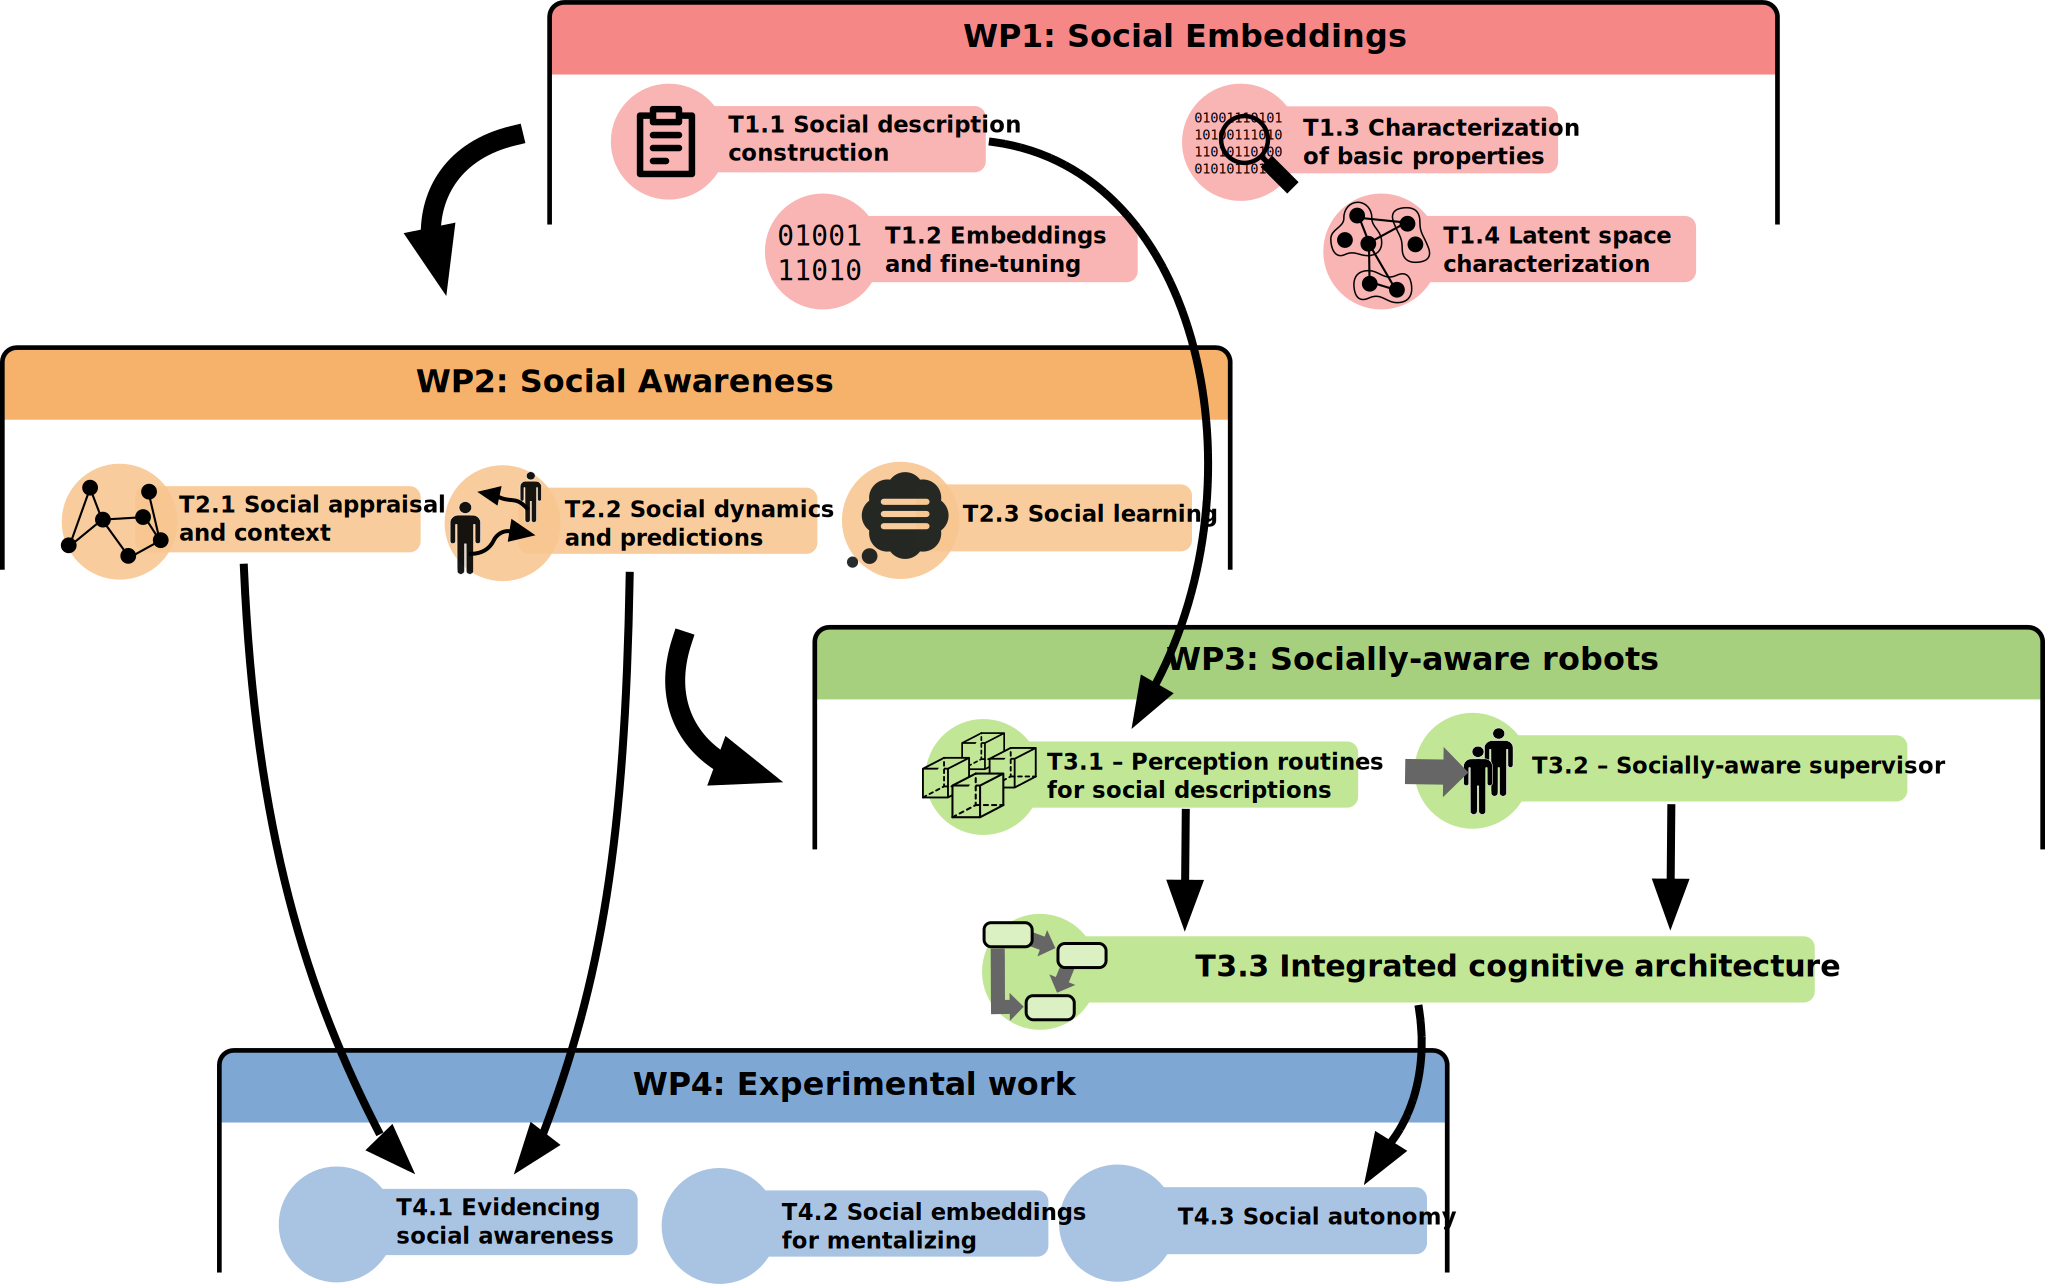
\includegraphics[width=\linewidth]{figs/wps}
\caption{Overview of the workpackages and tasks, and tasks inter-relations.}
\label{fig:wps}
\end{figure}

More specifically, Figure~\ref{fig:wps} gives an overview of the project
workpackages, and their interrelations. Fieldwork plays a central role in the
project, and appears in the centre of the figure. The first important field
deployment is a one-year experiment, taking place at the Bristol science centre
(T1.1). This `public-in-the-loop' experiment is analysed and lead to the
definition of core interaction principles (T1.2). These are in turn translated
into algorithmic models, guiding the social teleology of the cognitive
architecture (T4.1).

This first experiment is immediately followed by two other long-term
experimental deployments: a one-year deployment in one of Bristol's Special
Education Need (SEN) school (T5.1), followed by a one-year deployment at
Bristol's Children's hospital (T5.2). These two additional experiments are both
inputs for WP2 and WP3, and demonstrator for the robot socio-cognitive
architecture (WP4).

Specifically, workpackage WP2 research, develop, and integrate all the components
pertaining to the assessment of the spatio-temporal and social environment of
the robot. Reference interaction situations and the data required to support
this workpackage is directly drawn from the experimental fieldwork that will
take place at the same time in WP1 and WP5. The perceptual capabilities
delivered by WP2 are continuously integrated into the robot's cognitive
architecture (T4.3), iteratively improving the socio-cognitive performances of
the robot.

Workpackage WP3 looks into behaviour generation using machine learning (T3.2)
and non-verbal affective modalities (T3.3). T3.2 is data-intensive, and will use
datasets acquired during the field deployments (T1.1, T5.1, T5.2), as well as
lab-recorded dataset of social interactions. Similar to WP2, the capabilities
built in WP3 are integrated in the robot architecture in T4.3.

In addition to the integration of WP2 and WP3 capabilities, WP4 is also
researching and developing the socio-cognitive drives of the architecture. They
come both from T1.2 (as previously mentioned), and
human-in-the-loop/public-in-the-loop machine learning (T4.2). T4.2, in
particular, is tighly connected to the experimental fieldwork, where the
learning-from-end-users take place.

\end{rewrite}

\subsubsection{Integration sprints}

\project is a complex project, with numerous interdependencies between tasks.
To ensure the interdependencies are properly understood, and support effective
integration of the outputs of each workpackage, I will organise every 6 months,
and for the first 4 years, \textbf{integration sprints} (see Gantt diagram).
Integration sprints are one-week long integration retreat during which the whole
\project team gather and work together to effectively implement and test on the
robot the different components. In addition to providing regular `check points'
for the projects, they also set a stable schedule to deliver project components.

This methodology was used by the PI in  several previous projects (FP7 CHRIS
project, H2020 SPRING for instance), and had proved to be of great value to
ensure project-wide cohesion and steady progress.

The three integration sprints taking place before the beginning of the
experimental deployments (display as orange circles on the Gantt chart) are of
particular importance, and will be extended to ten days.


\subsubsection{Gantt chart}

%\begin{landscape}
\begin{figure}[!ht]
\resizebox{\linewidth}{!}{
    
\def\pgfcalendarmonthletter#1{%
\ifcase#1 J\or J\or F\or M\or A\or M\or J\or J\or A\or S\or O\or N\or D\fi%
}

\begin{ganttchart}[
        canvas/.append style={fill=none, draw=black!5, line width=.75pt},
        hgrid style/.style={draw=black!5, line width=.75pt},
        vgrid={*1{draw=black!5, line width=.75pt}},
        %vgrid={*1{black}, *{11}{black!5}}, % doesnt work for some reason
        x unit=.35cm,
        y unit chart=.65cm,
        time slot format=isodate-yearmonth,
        time slot unit=month, % pgfgantt >= 5.0
        %compress calendar, % pgfgantt < 5.0 => overleaf
        title/.style={draw=none, fill=none},
        title label font=\bfseries\footnotesize,
        %title label node/.append style={below=7pt},
        include title in canvas=false,
        bar label font=\mdseries\small\color{black!70},
        %bar label node/.append style={left=2cm},
        bar/.append style={draw=none, fill=barcolor!50},
        bar progress label font=\mdseries\footnotesize\color{black!70},
        group/.append style={fill=barcolor},
        group incomplete/.append style={fill=black},
        group left shift=0,
        group right shift=0,
        group height=.5,
        group peaks tip position=0,
        %group label node/.append style={left=.6cm},
        group progress label font=\bfseries\small,
        link/.style={-latex, line width=1.5pt, linkred},
        link label font=\scriptsize\bfseries,
        link label node/.append style={below left=-2pt and 0pt,
        milestone/.append style={circle},
        milestone inline label node/.append style={left=5mm}}
    ]{2026-01}{2030-12}
    
        %\gantttitle[
        %    title label node/.append style={below left=7pt and -3pt}
        %]{Month:\quad1}{1}
        %\gantttitlecalendar{year, month=letter} \\
        \gantttitlecalendar{year} \\
        %\gantttitlelist{0,5,...,60}{1} \\
        %% WP1
        \definecolor{barcolor}{RGB}{246,135,135}
        \ganttgroup[]{WP1 \wpA}{2026-01}{2029-06} \\
            \ganttbar[name=TAA]{\TAA}{2026-01}{2026-12} \\
            \ganttbar[name=TAB]{\TAB}{2026-07}{2027-06} \\
            \ganttbar[name=TAC]{\TAC}{2027-01}{2027-12} \\
            \ganttbar[name=TAD]{\TAD}{2028-01}{2029-06} \\
            %\ganttbar[name=WP12prep,inline,bar/.append style={fill=gray!20}]{preparation}{2026-07}{2026-12}
            %\ganttbar[name=WP12exp,inline]{WeTheCurious experiment}{2027-01}{2027-12}
            %\ganttbar[name=WP12]{\textbf{1.2} Principles of r-HHI}{2028-01}{2028-06} \\

        %\ganttlink[link type=f-s]{WBS1A}{WBS1B}

        %% WP2
        \definecolor{barcolor}{RGB}{246,178,107}
        \ganttgroup[]{WP2 \wpB}{2027-01}{2029-12} \\
            \ganttbar[name=TBA]{\TBA}{2027-01}{2027-12} \\
            \ganttbar[name=TBB]{\TBB}{2028-01}{2028-12} \\
            \ganttbar[name=TBC]{\TBC}{2029-01}{2029-12} \\
            %\ganttbar[name=WP21]{\textbf{2.1} Situation assessment}{2026-01}{2027-06} \\
            %\ganttbar[name=WP22]{\textbf{2.2} Human model}{2027-01}{2028-12} \\
            %\ganttbar[name=WP23]{\textbf{2.3} Interactions \& social groups}{2029-01}{2029-12} \\
            %\ganttbar[name=WP24]{\textbf{2.4} Social situation assessment}{2027-07}{2029-12} \\

        %\ganttlink[link type=f-s]{WP21}{WP24}
        %\ganttlink[link type=f-s]{WP22}{WP23}

        %% WP3
        \definecolor{barcolor}{RGB}{166,208,126}
        \ganttgroup[]{WP3 \wpC}{2026-07}{2029-12} \\
            \ganttbar[name=TCA]{\TCA}{2026-07}{2027-06} \\
            \ganttbar[name=TCB]{\TCB}{2027-07}{2028-06} \\
            \ganttbar[name=TCC]{\TCC}{2028-01}{2029-12} \\
            %\ganttbar[name=WP31]{\textbf{3.1} Behaviours baselining}{2026-07}{2027-12} \\
            %\ganttbar[name=WP32]{\textbf{3.2} Generative behaviours}{2028-01}{2028-12} \\
            %\ganttbar[name=WP33]{\textbf{3.3} Non-verbal behaviours}{2028-07}{2030-12} \\
            %\ganttbar[name=WP41]{\textbf{4.1} Social teleology}{2028-01}{2029-12} \\
            %\ganttbar[name=WP42]{\textbf{4.2} Human-in-the-loop ML}{2026-07}{2030-06} \\
            %\ganttbar[name=WP43]{\textbf{4.3} Integrated cognitive arch.}{2026-01}{2030-06} \\

        %% WP4
        \definecolor{barcolor}{RGB}{126,167,211}
        \ganttgroup[]{WP4 \wpD}{2026-07}{2030-12} \\
            \ganttbar[name=TDA]{\TDA}{2026-07}{2027-06} \\
            \ganttbar[name=TDB]{\TDB}{2027-07}{2027-12} \\
            \ganttbar[name=TDD]{\TDB}{2028-01}{2028-06} \\
            \ganttbar[name=TDCprep,inline,bar/.append style={fill=gray!20}]{preparation}{2029-01}{2029-06} 
            \ganttbar[name=TDC]{\TDC}{2029-07}{2030-06} 
            \ganttbar[name=TDCexpl,inline,bar/.append style={fill=gray!20}]{analysis}{2030-07}{2030-12} 

            %\ganttbar[name=WP51prep,inline,bar/.append style={fill=gray!20}]{preparation}{2027-07}{2027-12}
            %\ganttbar[name=WP51]{\textbf{5.1} SEN schools experiment}{2028-01}{2028-12} 
            %\ganttbar[name=WP51expl,inline,bar/.append style={fill=gray!20}]{analysis}{2029-01}{2029-06} \\
            %\ganttbar[name=WP52prep,inline,bar/.append style={fill=gray!20}]{preparation}{2029-01}{2029-06}
            %\ganttbar[name=WP52]{\textbf{5.2} Children's hospital experiment}{2029-07}{2030-06}

        %\ganttlink[link type=f-s]{WP41}{WP51}


        %\ganttlink[link type=f-s]{WBS1B}{WBS1C}
        %\ganttlink[link type=f-f,link label node/.append style=left]{WBS1C}{WBS1D}
        \ganttnewline[thick]

        \ganttmilestone{\bf\sc Ethics workshops}{2026-04}
        \ganttmilestone{}{2027-09}
        \ganttmilestone{}{2028-09}
        \ganttmilestone{}{2030-03} \ganttnewline[gray,dotted]


        \ganttmilestone{\bf\sc Integration sprints}{2026-06}
        \ganttmilestone[milestone/.append style={fill=orange, circle}]{}{2026-11}
        \ganttmilestone{\bf\sc Integration sprints}{2027-06}
        \ganttmilestone[milestone/.append style={fill=orange, circle}]{}{2027-11}
        \ganttmilestone{\bf\sc Integration sprints}{2028-06}
        \ganttmilestone{\bf\sc Integration sprints}{2028-12}
        \ganttmilestone[milestone/.append style={fill=orange, circle}]{}{2029-05}

        % separate years
        \ganttvrule{}{2026-12}
        \ganttvrule{}{2027-12}
        \ganttvrule{}{2028-12}
        \ganttvrule{}{2029-12}
        \ganttvrule{}{2030-12}


        \ganttvrule[vrule/.append style={orange, solid, thin}]{study @WeTheCurious}{2026-12}
        \ganttvrule[vrule/.append style={orange, solid, thin}]{study @SEN school}{2027-12}
        \ganttvrule[vrule/.append style={orange, solid, thin}]{study @Broca
        hospital}{2029-06}

\end{ganttchart}

}
\end{figure}
%\end{landscape}


\subsubsection{Project's milestones}

\begin{table}[h!]
    \centering
\begin{tabular}{@{}lccccccr@{}}
\toprule
\textit{\textbf{}}              & \textbf{Y1} & \textbf{Y2} & \textbf{Y3} & \textbf{Y4} & \textbf{Y5} \\ \midrule
\textit{MS1:...} &   & x  &    &   &    &  &   \\ 
\textit{MS2:...} &   &    & x  &   &    &  &   \\ 
\textit{MS3:...} &   &    &    & x &    &  &   \\ 
\textit{MS4:...} &   &    &    &   & x  &  &   \\ \bottomrule
\end{tabular}
    \caption{Project's milestones}
    \label{milestones}
\end{table}

\subsubsection{Engineering methodology}

\TODO{useful?}

\begin{rewrite}

Detail use of:
\begin{itemize}
    \item use of ROS2
    \item coding guidelines enforced with linters
    \item CI/CD for automatic code testing
    \item integration testing using DOcker/Docker compose
\end{itemize}

\end{rewrite}

%%%%%%%%%%%%%%%%%%%%%%%%%%%%%%%%%%%%%%%%%%%%%%%%%%%%%%%%%%%%%%%%%%%%%%%%%%%
\subsection{Expertise and Research team}
\label{research-team}

My expertise is primarily centered on cognitive robotics and human-robot social
interaction. My expertise in this field covers a broad spectrum, from basic
research in robotics (for
instance~\cite{lemaignan2014dynamics,lemaignan2015mutual}) and data-driven
socio-psychology
(including~\cite{lemaignan2014cognitive,irfan2018social,winkle2019effective,bartlett2019what}),
to technical contributions (for instance~\cite{lemaignan2010oro,
lemaignan2017artificial, lemaignan2018underworlds}), to extensive experimental
work (see below; for instance~\cite{hood2015cowriter,winkle2020couch,
lemaignan2022social}).

Over the last 4 years, I have re-focalised my work on \emph{data-driven HRI},
contributing several new large datasets of social
interactions~\cite{lemaignan2018pinsoro,sallami2020unexpected,webb2023sogrin},
developing new data analysis
techniques~\cite{bartlett2019what,webb2022measuring}, and demonstrating with my
students new applications of interactive machine learning to social
interactions~\cite{senft2016sparc,winkle2020couch,winkle2021leador}.  In
parallel, I progressively matured the idea of computing compact
\emph{embeddings} of social situations, until I recently published a first
breakthrough in that direction~\cite{lemaignan2024social} (to appear at IEEE/ACM
HRI'24). This ERC project is directly born from this multi-year endeavour
towards data-driven social sciences applied to embodied AI systems, and aims at
significantly accelerate research in this direction.

In particular, \project is the opportunity to gather an interdisciplinary team
of academics that would effectively complement my expertise, and ensure the
feasibility of the project.

Specifically, I intend to recruit:

\begin{itemize}

    \item  two researchers with expertise in data-driven
        socio-psychology (one senior post-doc PD1, one PhD student PHD1); these
        researchers will directly contribute to the human data acquisition,
        the interpretation of social embeddings in term of social situations,
        and the experimental work;

    \item two researchers with expertise in deep machine learning and large
        language models (one senior post-doc PD2, one PhD student PHD2); these
        researchers will contribute to the core implementation of social
        embeddings, including language model fine-tuning, as well as the
        analysis of the embedding space topology;

    \item one research in cognitive robotics (PhD student, PHD3); this
        researcher will focus on the effective integration of social
        embeddings into a larger cognitive architecture for social robots, able
        to autonomously drive interactions;

    \item one researcher in ethics of technology (post-doc
        level PD3); this researcher will lead the work on understanding social
        embeddings in terms of ethical and responsible research.
\end{itemize}

Table~\ref{time-allocation-team} provides an overview of the time allocation per
members of the team, over the course of the project.

\begin{table}[h!]
    \centering
\begin{tabular}{@{}lccccccr@{}}
\toprule
\textit{\textbf{}}              & \textbf{Y1} & \textbf{Y2} & \textbf{Y3} & \textbf{Y4} & \textbf{Y5} &  & \textbf{Total months} \\ \midrule
\textit{Séverin Lemaignan (PI)} & 1         & 1         & 1         & 1
    & 1         &  & 60                    \\ \midrule
\textit{Post-doc 1 (WP1)}       & 1           & 1           & 1           &             &             &  & 36                    \\
\textit{Post-doc 2 (WP2)}       & 1           & 1           & 1           & 1           &             &  & 48                    \\
\textit{Post-doc 3 (WP3)}       &             & 1           & 1           & 1           & 1           &  & 48                    \\
\textit{Post-doc 4 (WP3, WP5)}  & 1           & 1           & 1           & 1           & 1           &  & 60                    \\
\textit{PhD 1 (WP3, WP5)}       &             & 1           & 1           & 1           & 0.5         &  & 42                    \\ \bottomrule
\end{tabular}
    \caption{Full-time equivalent for the research team members\TODO{to update}}
    \label{time-allocation-team}
\end{table}


In addition, the host institution (INRIA Grenoble) will provide extensive
additional expertise on machine learning applied to robotics. I will specifically build on
my already established collaboration with Dr. Xavier Almeida-Pineda, head of the
RobotLearn research group. Dr. Almeida-Pineda is the coordinator of the EU H2020
SPRING project on social robotics for geriatric care, on which I collaborated
for the past two years.

Additional expertise, as well as access to one of my main experimental
environment, will be provided through a collaboration with Paris' public
hospitals (APHP) and specifically, with Dr. Maribel Pino, head of research at
Paris' Broca geriatrics hospital (Dr. Pino has extensive experience running
studies with social robots on the hospital' premisses).


%%%%%%%%%%%%%%%%%%%%%%%%%%%%%%%%%%%%%%%%%%%%%%%%%%%%%%%%%%%%%%%%%%%%%%%%%%%
\subsection{Workpackages}

\subsubsection{WP1: \textbf{\WPA}}

WP1 addresses Objective \textbf{O1}. I will first systematically investigate the
three steps of social embeddings construction, and then characterize the
resulting embeddings.


\paragraph{\TAA}

Social embeddings construction requires first to extract descriptors, then to
build complete textual descriptions, and finally to embed these descriptions.  I
will extract basic social descriptors using the ROS4HRI social perception
approach, as it formalize a multi-modal model of humans~\cite{lemaignan2022ros},
and run in real-time on current robots. I will augment these basic descriptors
with more complex percepts, including (1) descriptors of human-objects
interactions (HOI), using transformer-based techniques
like~\cite{iftekhar2022what} ; (2) affective
descriptors~\cite{vinciarelli2009social}, using e.g. facial expressions based on
facial action units classification~\cite{martinez2019automatic}; (3) group-level
interactions, including $f$-formations~\cite{setti2015fformation}, and group
activity recognition, using deep convolutional graph techniques like
ARG~\cite{wu2019learning}.

%(3) a novel contextual model of
%attention~\cite{ferrini2024percepts} that allows fine-grained assessment of what
%the person around the robot are focusing on.

The generation of textual descriptions consists in both the combination of
descriptors into textual \emph{snapshots} of the social environment at a
specific time, and the combination of these snapshots over time, to build a
textual description of complete situations with a time horizon of 10s to
25s~\cite{netanyahu2021phase}. I will initially build snapshots using text
templates, and then extend the methodology using techniques based on
social knowledge graphs~\cite{sap2019atomic} and propositional
logic~\cite{tsoi2022sean}. The combination of snapshots into social situations
will be developed with the help of the PHASE simulator and
dataset~\cite{netanyahu2021phase}, that includes a large number of annotated
social interaction sequences.

\begin{framed}
    {\noindent\bf Main outcomes of \tAA:} lorem ipsum 
\end{framed}

\paragraph{\TAB}

This task focuses on the text embedding process itself. Due to the fast pace of
progress in the LLMs landscape, it is likely that current methods (including
e.g.~\cite{reimers2019sentencebert,muennighoff2022sgpt}) will have been
superseeded by new methods. I will closely monitor advances in the domain,
especially on the question of semantic relatedness~\cite{thakur2021beir}, as
this is critical for social embeddings. I plan to also perform
fine-tuning~\cite{hadsell2006dimensionality} of the selected text embedders to
specialize them for social situation representation. I will do so by leveraging
existing open-access annotated datasets of social interaction like
AMI~\cite{carletta2007ami}, D64~\cite{oertel2013d64},
SALSA~\cite{alameda2015salsa}, or my own SoGrIn dataset~\cite{webb2023sogrin},
and datasets of social questions-answers like SocialIQa~\cite{sap2019social}.

\begin{framed}
    {\noindent\bf Main outcomes of \tAB:} lorem ipsum 
\end{framed}

    \paragraph{\TAC}

\begin{rewrite}
I will then characterise social embeddings, starting with the fundamental
properties that I identified in~\cite{lemaignan2024social}: invariance to
syntax, social similarity and continuity. 
\end{rewrite}

\begin{framed}
    {\noindent\bf Main outcomes of \tAC:} lorem ipsum 
\end{framed}

\paragraph{\TAD}

\TODO{rephrase; be more specific (eg cf Sun's paper)}

This task will look into the characterization of the embeddings' \emph{latent
semantics}: For instance, social descriptions like `two persons chatting and
laughing together'; or `a group of three people walking together'; or `one
single person walking towards the robot, looking agitated'; etc.  are all
semantically distinct, and, consequently, would belong to distinct regions in
the embedding space. Identifying such clusters to characterize the semantic
topology of the embedding space~\cite{sun2023topological} will be achieved by
exploiting existing annotated datasets to identify and extract prototypical
reference social situations.

\begin{framed}
    {\noindent\bf Main outcomes of \tAD:} lorem ipsum 
\end{framed}


\begin{framed}
    \noindent{\bf WP Timeframe:} Y1-Y3.5; one post-doc ({\bf PD1}) with expertise in
    deep learning/text embedding; one post-doc ({\bf PD2}) in data-driven
    sociology.
\end{framed}

\subsubsection{WP2: \textbf{\WPB}}

\emph{Social awareness} is a socio-cognitive skill that is essential for
artificial social system, like social robots, to e.g.  act in a
context-sensitive manner, reason and apply social norms, or create proactive
social agents (in order to acknowledge and respond to a human who would like
to engage with the robot, the robot must first adequately model and
recognise the corresponding social situation).

Work package WP2 focuses on research objectives \ref{T5}, \ref{T4} and \ref{T2}:
expanding social embeddings beyond their fundamental properties, to build a
`social awareness' cognitive skill for social robots.

\TODO{justify these 3 objectives}
\begin{itemize}
    \item appraise social situations, also taking into account the social context
    \item learn socially-appropriate behaviours
    \item anticipate future social states
\end{itemize}



\paragraph{\TBA}

The first task of this workpackage focuses on \emph{social appraisal}.

Social appraisal (Objective~\ref{T5}) is about interpreting the results of WP1
in terms of social situations\TODO{...}

Context-awareness is another critical aspect of social situation appraisal.
\emph{Context} has been defined in various way, including as \emph{who},
\emph{what}, \emph{when}, \emph{where}, and \emph{why} of
interactions~\cite{vinciarelli2009social}; as high-level task/environment
characteristics, such as `studying' or `dining'~\cite{nigam2015social}; as
relationships between agents in the scene, such as `interacting in a group',
`standing in a line'~\cite{althaus2004navigation}; or as
task-based~\cite{castellano2012detecting}. Social embeddings lend themselves
well to context encoding: as long as a context description can be generated, it
can be appended to the social situation description, and jointly embedded.
I will use \TODO{list context sources + algos: location, robot's role, on-going
task, etc}
%
%\emph{Characterizing} how context impacts the resulting social embeddings
%requires extensive research, from defining and specifying a taxonomy of
%contexts, to characterizing their impact on the social embedding space.

\TODO{need to be SMART: reference specific techniques + metrics}

This task is linked to the experimental task \TDB.


\begin{framed}
    {\noindent\bf Main outcomes of \tBA:} lorem ipsum 
\end{framed}

\paragraph{\TBB}

Objective~\ref{T4} and the learning of socially-appropriate behaviour
generation, \project aims at significantly advancing the state of the art in
this regard, by combining two techniques: (1) generative neural networks
for affective robot motion
generation~\cite{marmpena2019generating,suguitan2020moveae}; (2) interactive
machine learning in high-dimensional input/output spaces, where I have shown
with my students promising results for generating complex social
behaviours~\cite{senft2019teaching, winkle2020couch} that fully involve the
end-users~\cite{winkle2018social}. Modulating (1) with the social embedding of
the current situation will enable the generation of non-repetitive and socially
appropriate behaviours (gestures, motions, gazing behaviours, facial
expressions); augmenting the input space of (2) with social embeddings will
enable the robot to learn contextualised social policies

This task is linked to the experimental task \tDD.

\begin{framed}
    {\noindent\bf Main outcomes of \tBB:} lorem ipsum 
\end{framed}

\paragraph{\TBC}

This task looks onto how social embeddings can offer a novel approach to the
modelling and interpretation of \emph{social dynamics}. I hypothesise that
social dynamics correspond to \emph{trajectories} of social situations in the
embedding space.  For instance, the velocity in the embedding space should
reflect the rate of change of a social situation in the physical space;
trajectory extrapolation could be employed by robots to anticipate upcoming
social situations; discontinuities in the embedding space would reflect brutal
social changes that could trigger specific robot behaviours (for instance to
acknowledge or attempt to repair social situations).  \TODO{need to be SMART:
reference specific techniques + metrics}


\begin{framed}
    {\noindent\bf Main outcomes of \tBC:} lorem ipsum 
\end{framed}


\begin{framed}
    \noindent{\bf WP Timeframe:} Y2-Y4; one post-doc ({\bf PD3}) in cognitive
    sciences; one PhD student in data-driven sociology ({\bf PHD1}).
\end{framed}





\subsubsection{WP3: \textbf{\WPC}}

\begin{rewrite}

WP3 design and implement on the TIAGoPro robot the principled cognitive architecture
that binds together the socio-cognitive perceptual capabilities of the robot
(WP2), with its action production mechanisms (WP3).

\textbf{T3.1 -- A social teleology for robots}
\emph{Teleological systems} (ie goal-driven) has been investigated in robotics
for being a way of providing long-term drives to an autonomous robot. This has
been successfully applied to curiosity-driven robots~\cite{oudeyer2005playground} or motor babbling in infant-like
robots~\cite{forestier2017unified}, but only for relatively simple cognitive
systems. This task's objective is to define and implement a novel \emph{social teleology} that would
algorithmically encode long-term social goals into the robot. This will directly
build from the results of WP1, where interaction principles for social robots
are experimentally uncovered.

\begin{framed}
    {\noindent\bf Main outcomes of T3.1:} the algorithmic translation of WP1's
    interaction principles in long-term social goals for the robot, eg a
    long-term, socially-driven action policy for the robot.
\end{framed}

\textbf{T3.2 -- Learning from humans to achieve `by-design' responsible \&
trustworthy AI}
Building on my recent, promising results on human-in-the-loop
social learning~\cite{senft2019teaching,winkle2020couch}, this task
implements the learning mechanics (including the bi-directional interface
between the human teacher and the robot) to allow human end-users to
teach the robot domain-specific (at school, at the hospital) social policies,
following the methodology and the interactive reinforcement learning approach I
developed with my students in~\cite{senft2017supervised}.

In addition, this task will study through qualitative methods (thematic
interviews and questionnaires) how human-in-the-loop machine learning enables a more
trustworthy AI system, by involving the end-users in the creation of the robot
behaviours, thus offering a level of behavioural transparency to the end-users.

\begin{framed}
    {\noindent\bf Main outcomes of T3.2:} a human-in-the-loop reinforcement
    learning paradigm, suitable for in-situ teaching of the robot by the
    end-users themselves.
\end{framed}

\textbf{T3.3 -- Integrating a socially-driven architecture for long-term interaction}
This task builds on the state of art in cognitive architectures (disembodied
ones~\cite{chong2007integrated,vernon2007survey,kingdon2008review,duch2008cognitive,langley2009cognitive,taatgen2010past,thorisson2012cognitive},
as well as ones specifically developed for robotics:
ACT-R/E~\cite{trafton2013act}, HAMMER~\cite{demiris2006hierarchical}, PEIS
Ecology~\cite{saffiotti2005peis,daoutis2012cooperative},
CRAM/KnowRob~\cite{beetz2010cram, tenorth2009knowrob},
KeJia~\cite{chen2010developing}, POETICON++~\cite{antunes2016human}, and my own,
the LAAS Architecture for Social Interaction~\cite{lemaignan2017artificial}):
the overall purpose of the socio-cognitive architecture of \project is to
integrate in a principled way the spatio-temporal and social knowledge of the
robot (WP2) with a decision-making mechanism, to eventually produce
socially-suitable actions (WP3). 

The decision-making mechanism is the heart of the \project AI engine: the robot
will rely on it to generate action decision that are purposeful, legible and engaging on the
long run, something that none of the existing architectures have been able to
successfully demonstrate to date. I aim at a breakthrough, and will
introduce a novel approach: drawing from the interaction patterns identified
in T1.2, I will combine long-term, socially-driven goals (\emph{social teleology}, T3.1), and
human-in-the-loop machine learning (T3.2) using a novel arbitration mechanism.

to make ensure local adaptation  progressively learn an social
policy enabling long-term autonomy. This task focuses on `bringing the pieces
together' in a principled manner.


The arbitration mechanism itself will build on research on reinforcement
learning for experience transfer~\cite{madden2004transfer} that enables the
re-assessement of a policy (here, our long-term social teleology) based on
specific experience (here, the end-user-taught policy).


\begin{framed}
    {\noindent\bf Main outcomes of T3.3:} A cognitive architecture, implemented
    on the TIAGoPro robot, that enables long-term social engagement, by combining
    long-term goals with domain-specific action policies, taught by the
    end-users themselves.
\end{framed}

\end{rewrite}


\paragraph{\TCA}

lorem ipsum

\begin{framed}
    {\noindent\bf Main outcomes of \tCA:} lorem ipsum 
\end{framed}

\paragraph{\TCB}

lorem ipsum

\begin{framed}
    {\noindent\bf Main outcomes of \tCB:} lorem ipsum 
\end{framed}

\paragraph{\TCC}

lorem ipsum

\begin{framed}
    {\noindent\bf Main outcomes of \tCC:} lorem ipsum 
\end{framed}


\begin{framed}
    \noindent{\bf WP Timeframe:} Y1.5-Y4; one ... ({\bf PDx}) with expertise in
    ...; one ... ({\bf PDx}) in ...
\end{framed}











\subsubsection{WP4: \textbf{\WPD}}

\begin{rewrite}

\project has the ambition to demonstrate long-term, co-designed social
interactions in two complex, socially sensitive spaces.
The first one involves the deployment of social robots in special needs schools
(SEN schools) in Bristol (T5.1). Building on a rigorous participatory approach
involving the school teachers, as well as the parents, we will seek to integrate
the robot in the daily life of the school, supporting the development of the
students' physical and social skills. The second one takes place in Bristol's
Children's Hospital (T5.2), supporting isolated children who suffer long-term
conditions, in close cooperation with the hospital staff. In both cases, a
social robot will be deployed on premises, for one un-interrupted year. It will
integrate the daily routines of the institutions, under supervised
autonomy~\cite{senft2017supervised}, and \emph{without} requiring the
presence of a researcher at all time.

These two experiments raise specific practical and ethical questions, as they
target vulnerable populations. This is an however informed choice: first, I
already have established partnerships with Bristol's children hospital on one
hand, and a network of Bristol-based SEN schools on the other hand. As such, and
from a practical perspective, I do not foresee any institutional issues -- on
the contrary, our partners are excited at the prospect of taking part to the
project. Besides, convincingly demonstrating the importance and positive impact
of socially-driven, socially-responsible robotics does accordingly require
complex social situations, and complex social dynamics. The two scenarios, which
complement each other, provide both. These scenarios also put the project in the
unique position of actually delivering high societal impact: we anticipate 30+
hospitalised children with long-term conditions, and 250+ SEN-educated children
to directly benefit of the project, showing how robots can have a lasting,
beneficial impact on the society, alongside human carers: it will establish the
idea of \emph{robots supporting human interactions} instead of dehumanising our
social relationships.

Both these deployments will take place within the strict ethical framework
established in T1.1, the ethical considerations pertaining to these experiments
are further discussed below, in the section on ethics, and in the separate annex
on ethics, uploaded alongside this proposal.


\TODO{explain that these 2 large experiments will be scaffolded by many smaller
ones}

\textbf{T5.1: A robot companion to support physical, mental and social
well-being in SEN schools}

Inspired by a similar large-scale deployment of social robots in Hong-Kong's SEN
schools~\cite{robot4sen}, the first study investigate whether a socially
assistive robot can effectively support the development, social
interactions and well-being of children with a long-term mental condition. This
study will take place within the network of Bristol-based SEN schools, with
which I already have an on-going collaboration.  Specifically, the two main
questions we seek to investigate are: What are the social underpinnings of the
successful integration of a social robot in the school ecosystem? Can ambitious
co-design with the end-users (teachers) deliver a `net gain' for the learning,
social interaction and well-being of the students? 

The core of the study consists in deploying the R1 social robot in one of
Bristol-based SEN school (Mendip Primary School, with possible extensions to
other schools), to investigate how the robot can help shaping a social school
ecology that fosters mental well-being, while effectively supporting teachers
and students in their learning. 

The study will adopt a strong participatory design approach, inspired by
Patient and Public Involvement methodologies (PPI~\cite{boivin2010patient}),
with 3 one-day focus groups organised with the school teachers; two evening focus group with the
school parents, prior to the study; and several preparatory workshop at the
school premises to involve the students as well.

%During the first
%workshop, the teachers will be introduced to the robot capabilities with
%examples of robot-supported teaching activities, and the robot's visual
%programming interface will be introduced. We will also conduct group discussions
%on how the robot can best be integrated in the daily school routine and
%classroom context. During the second workshop, the teachers will be invited to
%create novel activities, with the support of the research team. An evening focus
%group will be organised as well with the parents, to integrate their
%perspectives in the design of the robotic system.  Will we formally analyse the
%data from this – will it become a research paper? 

%Following the workshops, the teacher-oriented codesign of the robot's activities
%and supervision tools (eg to start/stop/pause/resume activities) will be
%finalised and implemented by the research team.

The school study itself will take place during Y3, with the robot permanently
based at the school. The robot will take part in the
regular teaching and other daily routines of the school, and will directly
interact with the children, learning its action policy (`when to do what') from
initial co-design with the teachers, followed by progressive in-situ teaching (see
T4.2).

During selected `observation days', observations will be conducted by the
research team, and regular semi-structured interviews will be conducted with the
teachers, parents, and where possible, the children themselves (using engagement
metrics like the Inclusion of Other in Self task and Social-Relational
Interviews~\cite{westlund2017measuring}), to understand how the robot impacts
the school dynamics  (both positively and potentially negatively).

The task will be jointly supervised with local colleague and expert Dr.Nigel Newbutt,
who has a long track record of working with special needs schools.

\textbf{T5.2 -- A robot companion to support isolated children during their
hospital stay}

The second experiment will take place within the paediatric ward for long-term
conditions at the Bristol Children's Hospital. The ward has 8 beds, with
children staying from a few weeks to several years. Over the course of the
one-year deployment, we expect the robot to interact with about 30 children,
their parents, and the hospital staff (nurses, doctors).

Similar to the first experiment, we will be using a \emph{mutual shaping}
approach~\cite{winkle2018social} to design the role of the robot with the
different stakeholders (nurses, doctors, parents, children), in order to
experimentally investigate how a social robot can support hospitalised children
with long-term conditions. The robot's role will revolve around facilitating
social interactions between (possibly socially isolated) children, by fostering
playful interaction within the paediatric ward.

This second experiment complements the first one by evidencing the commonalities
and divergences in terms of social interactions when the robot is moved to a
different environment. While the hospital eco-system is comparatively smaller that the SEN school one,
people `live' at the ward day and night; it becomes \emph{de facto} the second home of the
children, and the children will have more interaction opportunities than at the
SEN school (where the robot is shared amongst a larger group). As a consequence,
we expect to observe different interaction patterns, with potentially deeper
affective engagement between the robot and the other ward's `inhabitants'.
Specific safeguarding measures will be put in place with the hospital team, and
resulting observations will feed into the ethical guidelines of T1.1.

\end{rewrite}


\paragraph{\TDA}

lorem ipsum

\begin{framed}
    {\noindent\bf Main outcomes of \tDA:} lorem ipsum 
\end{framed}

\paragraph{\TDB}

I will adapt to social
robotics~\cite{lemaignan2015mutual} experimental protocols originally designed
by Frith and Happé~\cite{frith1994autism} to investigate social representation
and mental modelling in autistic children.  This protocol include tasks like
distinguishing \emph{happiness} or \emph{sadness} from \emph{surprise}, or
distinguishing \emph{sabotage} from \emph{deception}: these nuances, quite
self-explanatory to experienced social agents, require subtle modelling of the
context and mental state of agents, and, until now, have not been successfully
reproduced on robots. I aim to show that social embeddings offer a generic
methodology to implement this kind of advanced social awareness.


\begin{framed}
    {\noindent\bf Main outcomes of \tDB:} lorem ipsum 
\end{framed}

\paragraph{\TDD}

lorem ipsum

\begin{framed}
    {\noindent\bf Main outcomes of \tDD:} lorem ipsum 
\end{framed}


\paragraph{\TDC}

lorem ipsum

\begin{framed}
    {\noindent\bf Main outcomes of \tDC:} lorem ipsum 
\end{framed}


\begin{framed}
    \noindent{\bf WP Timeframe:} Y1.5-Y4; one ... ({\bf PDx}) with expertise in
    ...; one ... ({\bf PDx}) in ...
\end{framed}


\subsubsection{WP5: \textbf{\WPZ}}

The last workpackage groups all the task related to the grant management, as
well as the dissemination and exploitation tasks.

The interdiscplinary nature of the project means that dissemination actions, in
particular, needs to target a broader range of practionners and stakeholders
than in typical projects.

\project has the ambition to disrupt how we study social interactions. While the
experimental side of the project is focused on applications in social robotics,
the impact of the project is not limited to this field, and I intend to
disseminate this work to a range of academic communities, from pure AI, to the
emerging field of data-driven sociology.


\paragraph{\TZA}

lorem ipsum

\begin{framed}
    {\noindent\bf Main outcomes of \tZA:} lorem ipsum 
\end{framed}

\paragraph{\TZB}

lorem ipsum

\begin{framed}
    {\noindent\bf Main outcomes of \tZB:} lorem ipsum 
\end{framed}

\paragraph{\TZC}

lorem ipsum

\begin{framed}
    {\noindent\bf Main outcomes of \tZC:} lorem ipsum 
\end{framed}


\begin{framed}
    \noindent{\bf WP Timeframe:} Y1.5-Y4; one ... ({\bf PDx}) with expertise in
    ...; one ... ({\bf PDx}) in ...
\end{framed}


%%%%%%%%%%%%%%%%%%%%%%%%%%%%%%%%%%%%%%%%%%%%%%%%%%%%%%%%%%%%%%%%%%%%%%%%%%%
\subsection{Experimental methodology}


%%%%%%%%%%%%%%%%%%%%%%%%%%%%%%%%%%%%%%%%%%%%%%%%%%%%%%%%%%%%%%%%%%%%%%%%%%%
\subsection{Towards Responsible Robotics research}

\begin{rewrite}

Because the development of socially-intelligent robots has
complex ethical ramifications -- including the potential of alienating
human users, \project also includes an explicit research component on
Responsible Robotics. In particular, the project will aim to contribute directly
to the on-going roadmap for Responsible Robotics, specifically
investigating the interplay between social embeddings, transparency and human
agency. The work will be conducted in workpackage WP4.


Social embeddings, by enabling artificial systems to model and reason on their
social environment, have the potential of significantly increase the social
competencies of e.g. robots, also raising ethical questions.

I am part of an international working group on Responsible Robotics~\TODO{cite
Dagsthul roadmap arxiv}...

%WP6 aims at establishing the conceptual and ethical framework around the idea of
%\emph{robot-supported human-human interactions}. It does so by co-creating
%patterns of interaction and norms with the general public, using a unique
%combination of ethnographic observations and `crowd-sourced' interaction
%patterns.
%
%\vspace{1em}
%\noindent\emph{Timeframe: Y3-Y5; one senior post-doc (PD3)
%with background in ethics of technology and responsible innovation.}




The \project project involves social robots, interacting in repeated ways and
over long period of time, with human end-users, including vulnerable children.
This raises complex ethical issues, both practical ones (how to design the
\project studies in a such a way that they are safe and ethically sound), and
more fundamental ones (what is the ethical framework for robots intervening in
socially sensitive environment?).



\subsection{Background on social robotic ethics}\label{ethics}

The ethical questions raised by social robotics have been actively studied over
the last 5 years, attempting to address issues like:

\begin{itemize}
    \item how to ensure that social robots are not used to simply replace the human
        workforce to cut costs?
    \item can we provide guarantees that the use of social robots will always be
        ethically motivated?
    \item further on, can we implement some ethical safeguarding built-in
        the system (like an ethical \emph{black-box}~\cite{winfield2017case})?
    \item what about privacy? how to trust robots in our home or school or
        hospital not to eavesdrop on our private lives, and, in the worst
        case, not be used \emph{against} us?
\end{itemize}

These questions are indeed pressing. The recent rise of personal assistants like
Amazon Alexa or Google Home, with the major privacy concerns that accompanies
their deployments in people home, shows that letting the industry set the agenda
on these questions is not entirely wise -- and robots can potentially be much
more intrusive than non-mobile smart speakers.  The EU is positioning itself at
the forefront of those questions. The recent release of operational \textbf{Ethics
Guidelines for Trustworthy AI} by the EU High-level Expert Group on Artificial
Intelligence~\cite{eu2019ethics} is a strong sign of this commitment. These
guidelines identify seven requirements of trustworthy AI:

\begin{enumerate}[label=\textbf{R\arabic*}]
    \item \textbf{Human agency and oversight}, including
            fundamental rights, human agency and human oversight

    \item \textbf{Technical robustness and safety}, including resilience to
        attack and security, fall back plan and general safety, accuracy,
        reliability and reproducibility

    \item \textbf{Privacy and data governance}, including respect for privacy,
        quality and integrity of data, and access to data

    \item \textbf{Transparency}, including traceability, explainability and
        communication

    \item \textbf{Diversity, non-discrimination and fairness}, including the
        avoidance of unfair bias, accessibility and universal design, and
        stakeholder participation

    \item \textbf{Societal and environmental wellbeing}, including
        sustainability and environmental friendliness, social impact, society
        and democracy

    \item \textbf{Accountability}, including auditability, minimisation and
        reporting of negative impact, trade-offs and redress.

\end{enumerate}

The design methodologies and techniques employed in \project naturally implement
most of these requirements: interaction co-design and human-in-the-loop machine
learning ensures human agency oversight over the robot's behaviours (R1);
Privacy and data governance (R3) is addressed in the project's data management
plan and facilitated by the design decision of performing all data processing
on-board the robot, avoiding the dissemination of personal information; the
transparency of the robot behaviour (R4) stems from the machine learning
approach that we advocate: the robot's behaviours primarily originate from what
the end-users themselves taught the robot; diversity and non-discrimination (R5)
is supported by the large-scale involvement of the public at the science centre,
ensuring a broad diversity of backgrounds and profiles; societal wellbeing (R6)
is the core research question of the project, and \project will contribute in
realising this requirement in the context of social robots.

Technical robustness (R2) and accountability (R7) are important design
guidelines for the robot's cognitive architecture (WP4), and will be addressed
there as well.


The Ethics Guidelines for Trustworthy AI form a solid foundation for the
project. However, personal and social robots raise additional questions
regarding what ethical and trustworthy systems might look like, and while the
principles of responsible design are somewhat established~\cite{stahl2016ethics,
bsi2016robots}, the reality of robot-influenced social interactions is not
fully understood yet, if only because the technology required to experience such
interactions is only slowly maturing. 

Social robots have indeed two properties that stand out, and distinguish them
from smart speakers, for instance.  First, they are fully embodied, and they
physically interact with their environment, from moving around, to picking up
objects, to looking at you; second, willingly or not, they are ascribed
\emph{agency} by people. This second difference has far-reaching consequences,
from affective bonding to over-trust, to over-disclosure of personal, possibly
sensitive, informations~\cite{martelaro2016tell,shiomi2017robot}.  As an
example, a common objection to human-robot interaction is the perceived
deceptive nature of the robot's role. It has been
argued~\cite{biscontilucidi2018companion} that the underlying concern is likely
the lack of an adequate (and novel) model of human-robot interactions to refer
to, to which the project will provide elements of response. This needs
nevertheless to be accounted for in depth.

Ethical framing of social robotics has started to
emerge under the term \textbf{roboethics}: the ``subfield of applied ethics
studying both the positive and negative implications of robotics for individuals
and society, with a view to inspire the moral design, development and use of
so-called intelligent/autonomous robots, and help prevent their misuse against
humankind.''~\cite{allen2011robot}. Specific subfields, like assistive
robotics~\cite{sharkey2012granny}, have seen some additional work, but social
robotics is still not equipped with operational guidelines, similar to the EU
guidelines on trustworthy AI.

\subsection{\project-specific measures}

I have chosen to focus the first workpackage task (T1.1) on building an
operational ethical framework for social robots which engage over long period of
time with the public. This work will deliver initial guidelines -- strongly
inspired by the guidelines on Trustworthy AI -- that will both form the ethics
basis for the \project experimental fieldwork, and have an impact beyond the
project, to feed into future European-level guidelines.

This work will be supported by an Ethics Advisory Board, composed of 3 experts
in ethics and social robotics and AI. While the exact composition of the board
is not final yet, it will include at least one member from the EU High-Level
Expert Group on Artificial Intelligence, that will be able to share the EU
expertise in framing ethics guidelines.

Practically speaking, these guidelines will form the basis of the ethics
approval process for the three long-term \project studies. It will be
additionally supported by my extensive experience in seeking ethics approval for
studies involving robots and vulnerable populations (in particular,
children~\cite{lemaignan2016learning,lemaignan2018pinsoro,senft2019teaching}),
the expertise of Dr. Newbutt in conducting research with SEN schools (T5.1), and
the support of J. Bowyer at the Bristol's Children's Hospital to obtain NHS ethics
approval. \textbf{As per requested, details of the ethics approval process,
children safeguarding, research Code of Conduct, and Data Management Plan are
annexed to the project proposal, in a separate `Ethics and Data Protection'
document}.

The project will also follow the European Commission recommendations for
Responsible Research and Innovation (RRI). RRI is defined
in~\cite{stilgoe2013developing} (and has been subsequently adopted by the UK Engineering
and Physical Sciences Research Council~\cite{owen2014uk}) using the acronym
AREA: Anticipation, Reflection, Engagement and Action. The \project research
will be undertaken responsibly by (1) \ul{Anticipating} possible consequences;
(2) by integrating mechanisms of \ul{Reflection} about the conducted work and its
aims; (3) by \ul{Engaging} with relevant stakeholders (general public, teachers,
hospital staff, parents, children themselves); and (4) by \ul{Guiding} action of
researchers accordingly. This approach has been formalised in the AREA 4P
framework~\cite{stahl2018implementing}~\footnote{\url{https://www.orbit-rri.org/about/area-4p-framework/}},
that I will use to guide the research strategy over the course of the project.
An additional role of the Ethics Advisory Board will be to advise and audit the
project with regards to this framework for responsible research.

\end{rewrite}



%%%%%%%%%%%%%%%%%%%%%%%%%%%%%%%%%%%%%%%%%%%%%%%%%%%%%%%%%%%%%%%%%%%%%%%%%%%
\subsection{Risk/gain analysis}

\begin{rewrite}

\textbf{Tasks 1.1, 1.2} develop a novel methodology, `public-in-the-loop' machine
learning, for large-scale co-design of social interactions with the public. If
successful, this will be of great value, well beyond the project. The
proposed experimental setup (science centre visitors `taking control' of the robot)
might however lead to interactions that are either too short or to artificial to
create meaningful, generalisable social interaction. In addition, the messy and
complex nature of the science centre environment is also currently beyond-state-of-the-art
in term of extracting the useful social features required to train a classifier.

However, the interaction principles that we want to uncover in T1.1 and T1.2
(and that are feeding into WP2 and WP4) will principally come from a qualitative
analysis of the interactions, carried in parallel to the machine learning
approach. This well within the expertise of the PI, and, as such, is low-risk.
T1.1 can thus be described as a \ul{\bf medium-risk, high-gain} component of
\project.

\vspace{1em}

\textbf{Task 2.1} develops a novel situation assessment component, that
integrates spatio-temporal modeling with knowledge representation. The resulting
component is beyond-state-of-the-art, and would be highly relevant to a large range
of robotic applications. This component relies on integrating tools that are
independently relatively mature and well understood, and the principles of the
integration itself is already well researched. Besides, it falls well within the
PI
expertise~\cite{lemaignan2018underworlds,sallami2019simulation,lemaignan2010oro}.
As such, T2.1 can be described as \ul{\bf low-risk, medium-gain}.

\textbf{Tasks 2.2, 2.3, 2.4} Work on real-time modeling of social dynamics in
real-world environments are only begining to be studied in robotics. While the
underpinning are well understood in neighbouring academic fields, a very
significant work remain to be done to integrate disparate or partial approaches
into one framework. These tasks also require the acquisition of novel datasets
that focus on natural human-human social interactions. The PI has extensive
experience in building and acquiring such
datasets~\cite{lemaignan2018pinsoro,sallami2020unexpected}, and does not
foreseen major difficulties. The resulting components have however the potential
to unlock a new class of social robots, aware in real-time of their social
surroundings and dynamics.  These tasks are thus considered \ul{\bf low-risk,
high-gain}.

\vspace{1em}

\textbf{Task 3.1} The behavioural baseline implements the current state-of-the-art,
and as such is \ul{\bf low-risk, low-gain}. T3.1 will guarantee early on in the
project a `working' robot, yet with predictable/repetitive behaviours.

\textbf{Task 3.2} The neural generation of complex social behaviours is a
\ul{\bf medium-risk, high-gain} task: while it builds on solid existing
state-of-the-art, it relies on very significant progress in both the modeling of the
social dynamics (WP2) and the capacity of designing a machine learning approach
to learn and generate these complex behaviours. While the former falls well
within the PI expertise, machine learning for social motion generation is
essentially a novel field. The success of this task will rely to a large
extend on the quality of the post-doctoral researcher recruited to lead this
effort. The main mitigation to the risk associated to T3.2 is the behavioural
baseline created in T3.1: the behavioural capabilities generated in T3.2 can be
complemented by ad-hoc behaviours whenever required.

\textbf{Task 3.3} Non-verbal communication is a well established subfield of HRI
research, well known to the PI. The creation of the novel interaction modality
based on soundscape is novel, with potential for impact beyond the project. This
new modality will be co-developped with an expert of sound design for
interaction, and we do not foresee major risks. Overall, the task is \ul{\bf
low-risk, medium-gain}.

\vspace{1em}

\textbf{Task 3.1} The conceptual framing of a \emph{socially-driven
architecture} (social teleology) and its translation into decision-making
algorithms are to a large extend open questions. This task might however lead to
uncover a fundamental mechanism to enable long-term engagement of users
with social robots. Building fundamentally on blue-sky research, this task is
\ul{\bf high-risk, high-gain}. If not successful, I will instead rely on the
decision-making strategy of T3.2, which is much lower risk.

\textbf{Task 3.2} The techniques developed in T3.2 have been previously used and
tested by the PI in two different real-world
environments~\cite{senft2019teaching,winkle2020couch}. While they will require
significant adjustments for this project, the task is overall \ul{\bf low-risk,
low-gain}.

\textbf{Task 3.3} The integration of the different cognitive functions of the
robot into one principled cognitive architecture, that include cognitive
redundancy, is one of the core expertise of the
PI~\cite{lemaignan2017artificial}. This task however includes significant novel
elements (cognitive mechanisms for long-term autonomy; decision arbitration)
that bear unknowns. Besides, this task is a critical pre-requisite for WP5. As a
result, T3.3 is considered as \ul{\bf high-risk}. The task is focused on
integration to meet the requirements of the WP5 experiments, and parts
of the resulting software architecture might be project-specific. However the
overall aims of endowing the robot with long-term social autonomy would be a
significant breakthrough, and as such, T3.3 is \ul{\bf high-gain}. The main
mitigations comes from (1) the iterative development process of the
architecture, that will start from the existing state-of-the-art, to which the
PI has previously contributed~\cite{lemaignan2017artificial}. By doing so, a
decisional architecture for the robot will be available early on in the project.
While that architecture might be a scaled-down version of the initial ambition,
it will still enable the fieldwork proposed in WP5, possibly with a lesser level
of autonomy; (2) the possibility of using only one of the two action policies
(T3.1 \ul{or} T3.2), thus removing the need for complex arbitration.

\vspace{1em}

\textbf{WP5: Experimental deployments}

The two application scenarios (at the children hospital and in the SEN school)
are ambitious and inherently risky, as they target vulnerable populations.
However, first, demonstrating the importance of advanced social modelling, and
convincingly proving the effectiveness of our approach does require accordingly
complex social situations, and complex social dynamics. The two scenarios, which
complement each other, provide both.

Second, working with vulnerable populations, in constrained and complex
environments (children hospital and SEN schools) adds significant risks to the
project. But it is also what make the project in the unique position of
delivering a high societal impact: a direct positive impact on children's lives
(we anticipate 100+ hospitalised children and 50+ children with psycho-social
impairements interacting over long periods of time with a robot over the course
of the project), and a broader impact on the society, showing how robots can
have a lasting, strong, positive impact on the society, also establishing the
idea of \emph{robots supporting human interactions} instead of dehumanising our
social relationships.

\textbf{Together, Task 5.1 and 5.2 are \ul{high-risk, high-gain}.}

The two main mitigations are (1) early and continuous engagement with the
stakeholders, and (2) the decoupling of the two applications, meaning that the
risks associated to each of them do not impact the other one.

Early engagement will be ensured by relying on a participatory design
methodology, involving all the stakeholders from the onset of the project; the
methodology will involve regular joint workshops; on-site (hospital and SEN
schools) research stay including engagement with the staff/charities and the
children themselves; early field testing and prototyping, relying if necessary
on provisional, yet well-known, robot platforms available at the host
institution (for instance, Softbank Nao and Pepper). This user-centered approach
will be championed by the post-doc recruited on the project on WP4 and WP5, who will
have to have a strong expertise in user-centered design.

It is also important to note that, while preparing this bid, initial discussions
have been held with all the partners involved with the experimental fieldwork
(WeTheCurious science centre, Bristol's Children Hospital, the network of SEN
schools): each of these institutions is enthusiastic about the project, already
contributing ideas to integrate the robots in their daily routines, and
ready to dedicate time and effort for its success.


\end{rewrite}




%%%%%%%%%%%%%%%%%%%%%%%%%%%%%%%%%%%%%%%%%%%%%%%%%%%%%%%%%%%%%%%%%%%%%%%%%%%
\newpage
\printbibliography



\end{document}
